\documentclass{article}   

\usepackage{geometry}
\usepackage{qtree}
\usepackage[square,numbers]{natbib}
% \usepackage{cite}  
\geometry{a4paper}

\usepackage[utf8]{inputenc}
\usepackage[T1]{fontenc}    % use 8-bit T1 fonts
\usepackage{lmodern}
\usepackage{hyperref}       % hyperlinks
\usepackage{lipsum}

\usepackage{color, colortbl}

\definecolor{Gray}{gray}{0.9}

\usepackage[protrusion=true,expansion=true]{microtype}

\usepackage{amssymb}
\usepackage{amsfonts}
\usepackage{eqnarray,amsmath}
\usepackage[table]{xcolor}

\usepackage{listings}
\usepackage{graphicx}
\usepackage{dirtytalk}

\usepackage[table]{xcolor}
\usepackage{rotating}
\usepackage{caption}

%% if you use PostScript figures in your article
%% use the graphics package for simple commands
\usepackage{graphics}


%% or use the graphicx package for more complicated commands
\usepackage{graphicx}
\usepackage[table]{xcolor}

\usepackage{indentfirst}
\usepackage[utf8]{inputenc}
 \usepackage{subcaption}
\usepackage{listings}
\usepackage{xcolor}
 
\definecolor{codegreen}{rgb}{0,0.6,0}
\definecolor{codegray}{rgb}{0.5,0.5,0.5}
\definecolor{codepurple}{rgb}{0.58,0,0.82}
\definecolor{backcolour}{rgb}{0.95,0.95,0.92}
 
\lstdefinestyle{mystyle}{
    backgroundcolor=\color{backcolour},   
    commentstyle=\color{codegreen},
    keywordstyle=\color{magenta},
    numberstyle=\tiny\color{codegray},
    stringstyle=\color{codepurple},
    basicstyle=\ttfamily\footnotesize,
    breakatwhitespace=false,         
    breaklines=true,                 
    captionpos=b,                    
    keepspaces=true,                 
    numbers=left,                    
    numbersep=5pt,                  
    showspaces=false,                
    showstringspaces=false,
    showtabs=false,                  
    tabsize=2
}
 
\lstset{style=mystyle}
% please place your own definitions here and don't use \def but
% \newcommand{}{}
%
% Insert the name of "your journal" with
% \journalname{myjournal}
%
\begin{document}

\title{%
  Practice 3: Gutenbergr project. \\~\\
  \Large Histograms}
\author{Mayra Cristina Berrones Reyes 6291}

\maketitle

\section{Introduction}

The Gutenberg Project is an online library that offers its users free access to more than 60,000 free books in different formats that go from ebooks, html, plain text, etc. It began with creator Michael Hart in 1971 at the Materials Research Lab at University of Illinois \cite{guten}.\\

In previous work, we explored some of the features of libraries for text analysis such as \texttt{gutenbergr, tidytext, tm,} and, \texttt{ dplyr}. Going deeper in analysis we now explore the sentiment analysis of texts using the library of \texttt{tidytext} to perform other experiments using histograms as a tool.\\

\section{Books}

Again for this project we use a book from the acclaimed novelist Jane Austen \cite{austen}, \textit{Pride and Prejudice} \cite{pride} published in 1813. And to make contrast in the present study, we are going to be comparing results with another book from another famous female author from the 19th century. \\

\textit{Wuthering Heights} \cite{wuhe} is a novel by the author Emily Bont$\ddot{e}$ \cite{emily} published in 1847. Her work is now regarded as classic in English literature, but in her time, the way she depicted mental and physical cruelty so attached to the love story she constructed in her book, challenged several Victorian ideas about religion, morality and class. \\

This two books are so alike in the way it changed public perception about class and the woman's place in society in their time, but their themes and tone of writing sound and feel to the reader so polarizing. So it gives us the focus for this experiment. Using the sentiment analysis of the library \texttt{tidytext}, we work to find the frequency of positive and negative words in both books.\\

\section{Data exploration}

To begin the exploration of the data, we start by tokenizing the words of each work. In Figure \ref{fig1} we see that there is not much difference in the use of what is known as stop words. The main distinct feature of this, is that in the work of Bront$\ddot{e}$ Subfigure \ref{subfig1-2} we have more of this connective words than in Subfigure \ref{subfig1-1} which is the Austen book.\\ 


\begin{figure}[]
\begin{subfigure}{.5\textwidth}
  \centering
  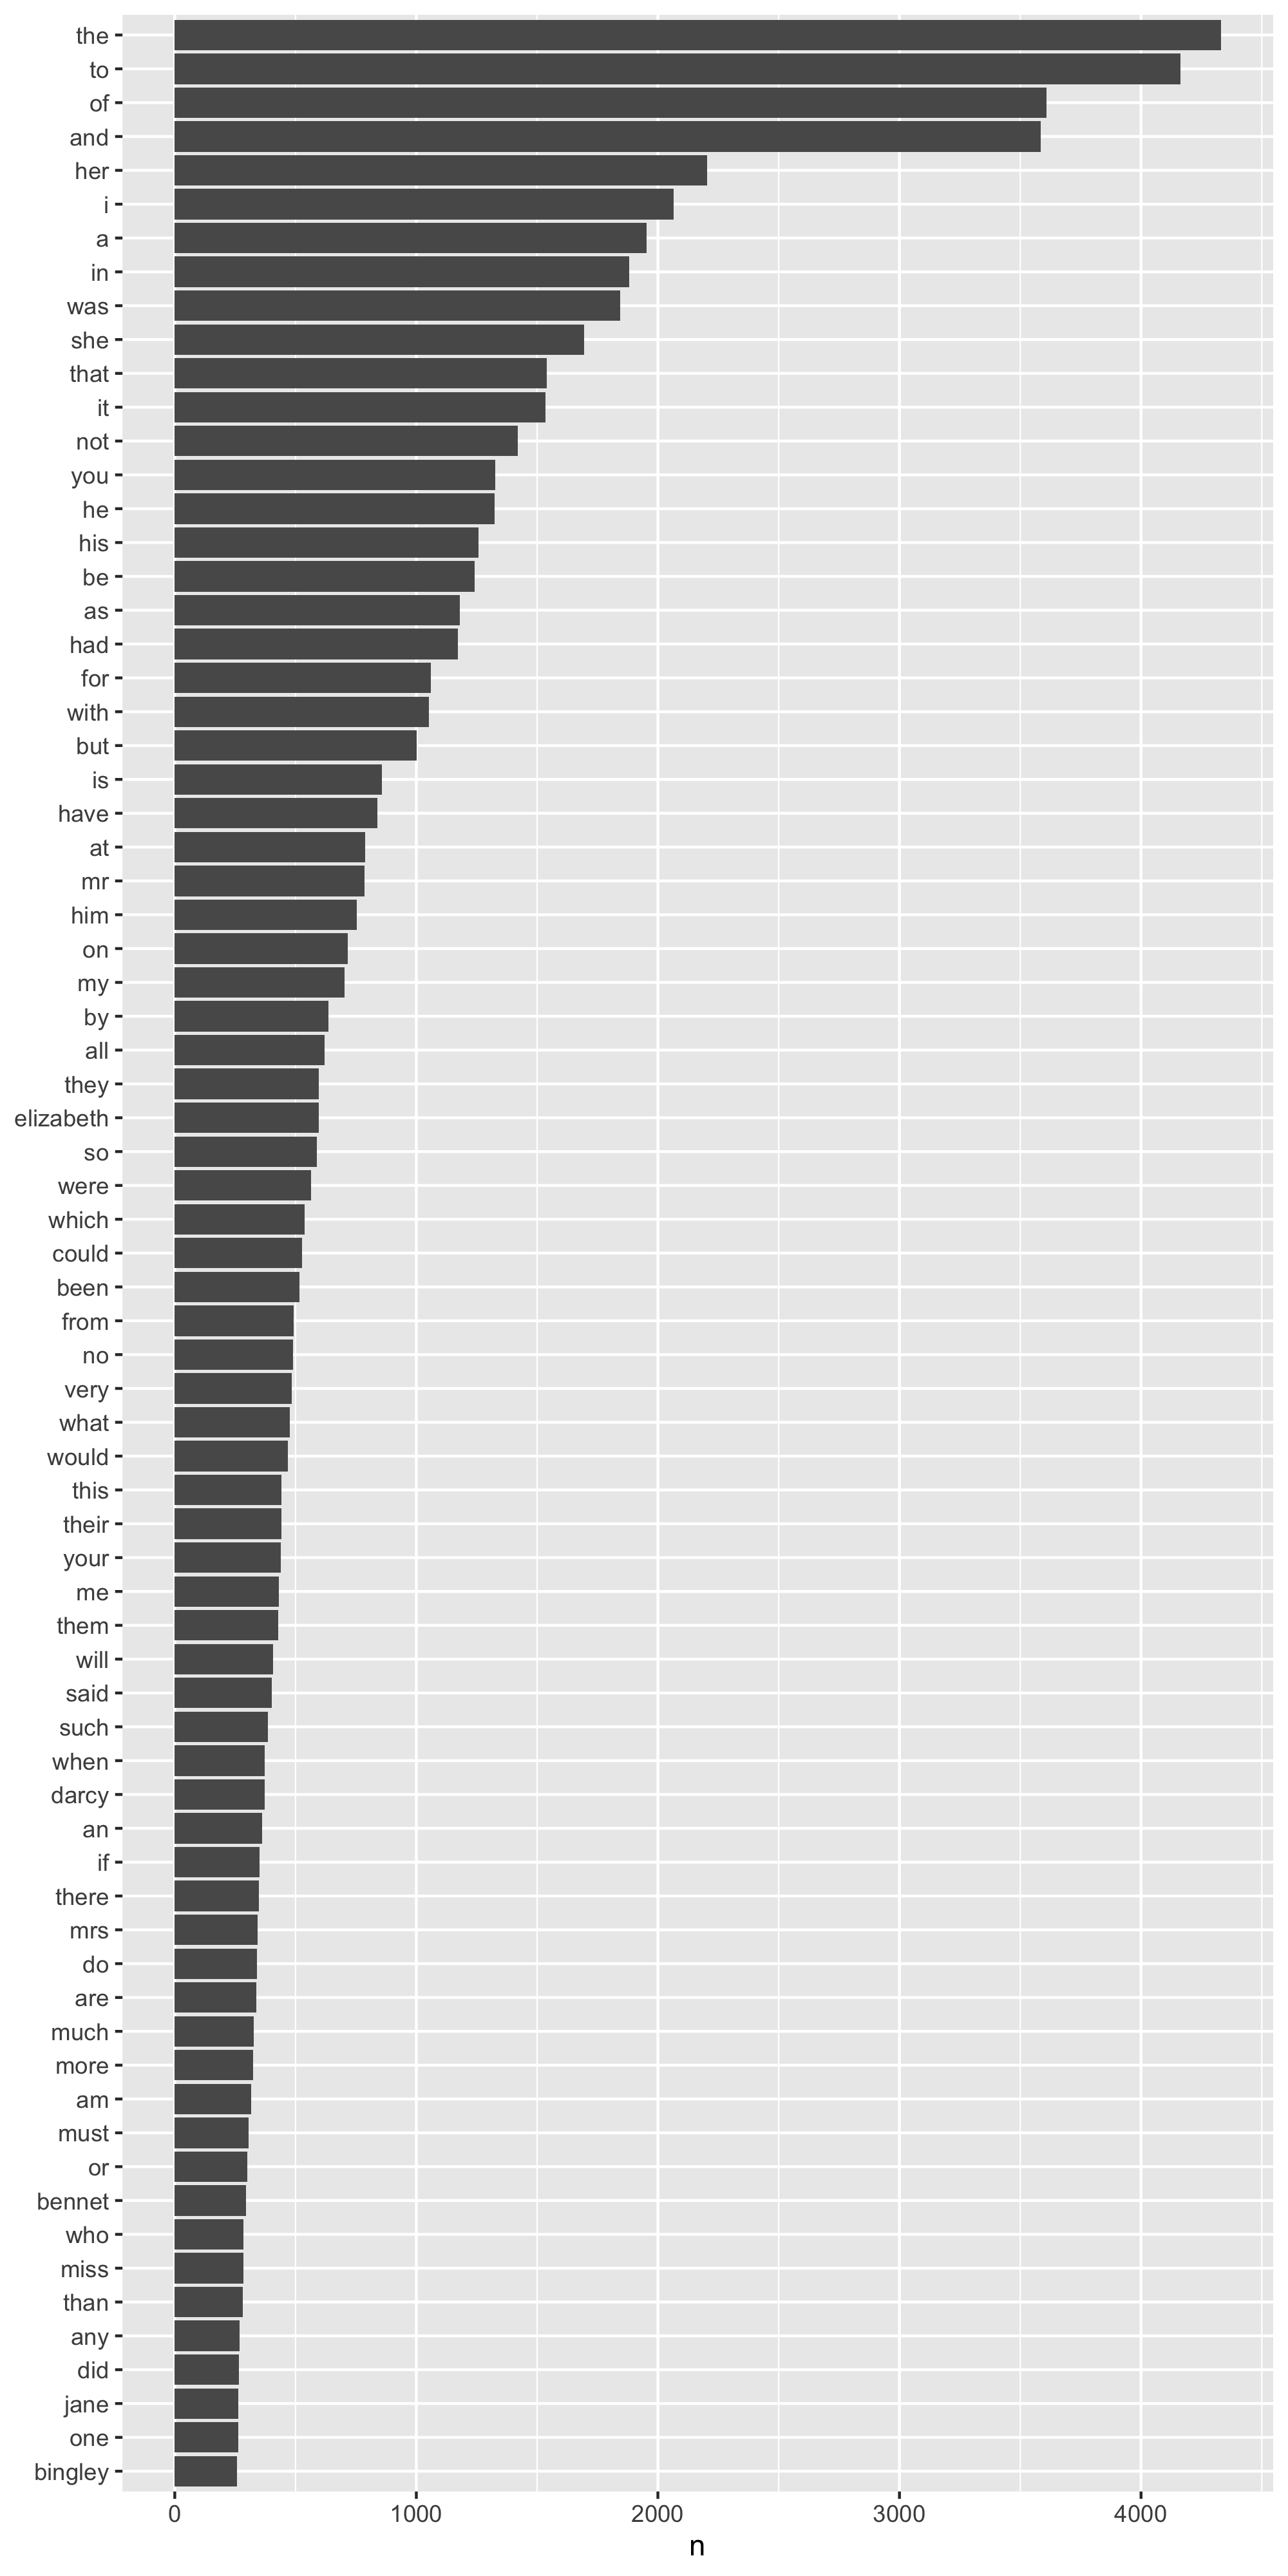
\includegraphics[width=1\linewidth]{Ej3.png}  
  \caption{Pride and Prejudice.}
  \label{subfig1-1}
\end{subfigure}
\begin{subfigure}{.5\textwidth}
  \centering
  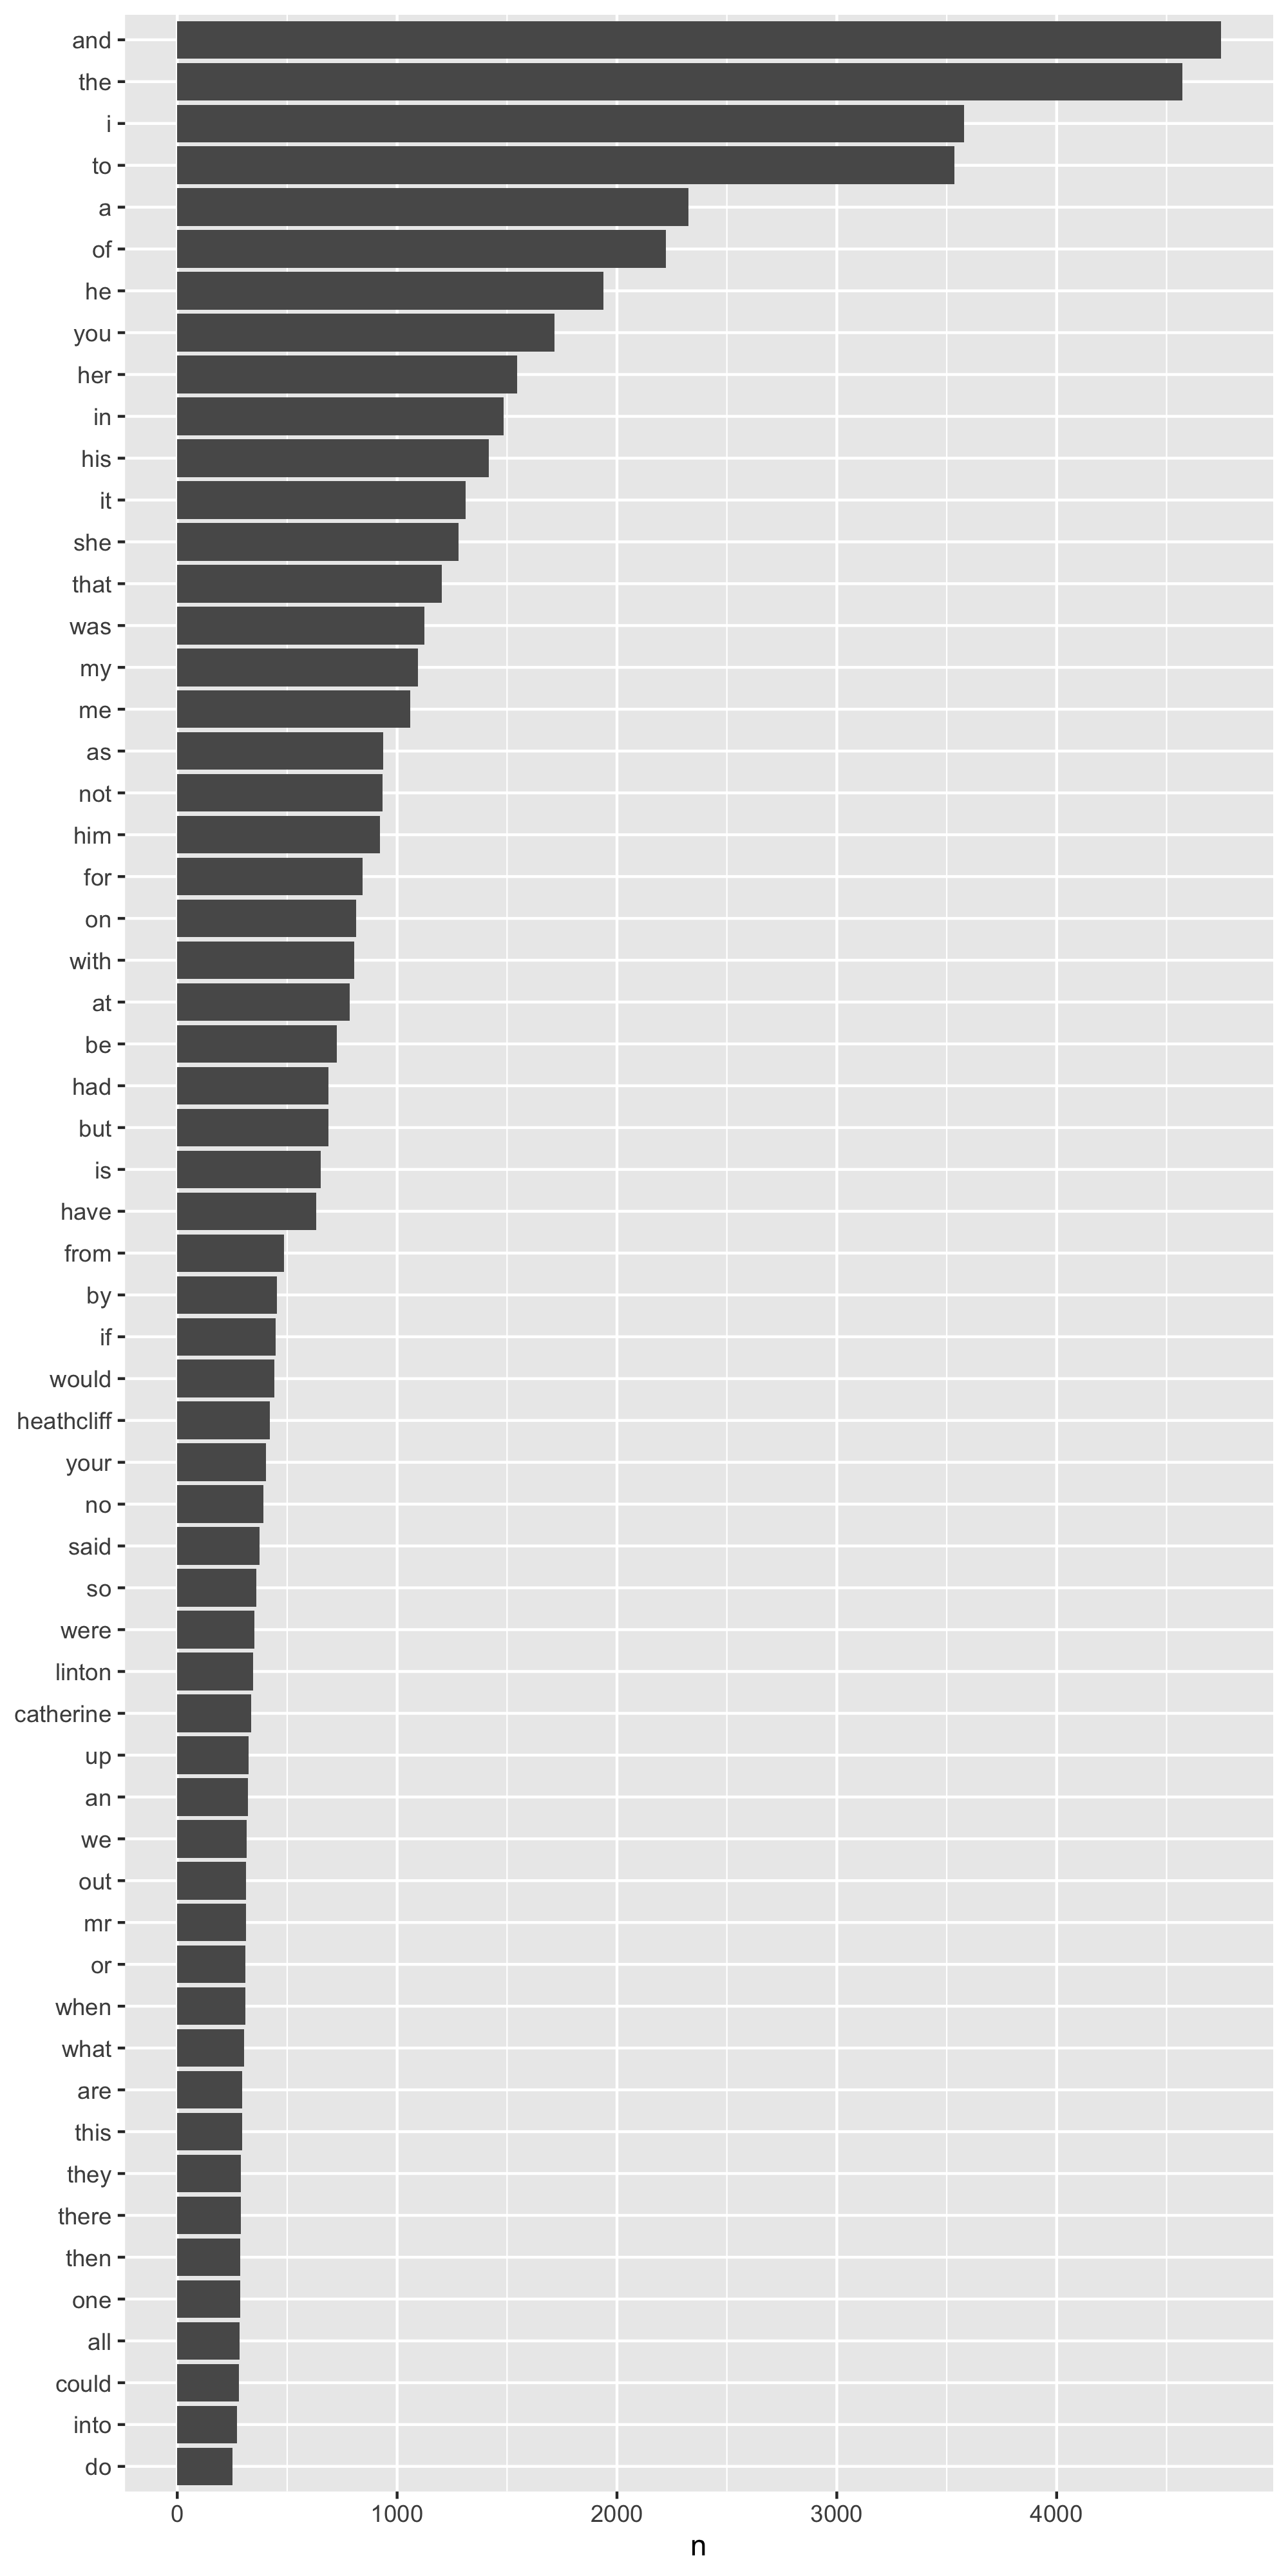
\includegraphics[width=1\linewidth]{Ej32.png}  
  \caption{Wuthering Heights}
  \label{subfig1-2}
\end{subfigure}
\caption{Frequency of all words in both books.}
\label{fig1}
\end{figure}

\clearpage

With this Figure \ref{fig1} we can assess that Bront$\ddot{e}$ is more prone to use connective words in her work. We can easily see that most of the words used on both books are similar in nature, except for the names of the characters. This can be associated with the fact that both authors are from the same era, and they both use British English.\\

Stop words however are not the main interest of the experimentation. The next step, in order to use the sentiment library is to create another variable without the stop words. This can be accomplished with the same library we used to tokenize the words on the downloaded document, only this time, we add the \texttt{anti join} variable. Inside we put \texttt{stop words} which is a data frame that contains pre loaded connective words in the English language.\\


Having the data free of stop words, we can now use the library of sentiment to analyse both books. There are a few libraries of sentiment in the \texttt{tidytext} library, but in this case we choose the \texttt{bing} because it manages the words into positive or negative emotions. In Figure \ref{fig2} the Subfigure \ref{subfig2-1} represents the positive and negative words of the book \textit{Pride and Prejudice}, and the same is represented in Subfigure \ref{subfig2-2} for the \textit{Wuthering Heights} book.\\

Right away when comparing the two Subfigures we notice that the negative words form the Austen novel have the feeling of being quite benign as opposed to the negative words in the Bront$\ddot{e}$ book. For instance, in textit{Pride and Prejudice} we have words like danger, poor, lost, absence, concern, dislike. And on the other hand in \textit{Wuthering Heights} we have words like dead, hate, dark, hurt, devil.\\

In the side of the positive words, we see how the distribution of the frequency of the words is smaller in the Bront$\ddot{e}$ side. Also, the top word \textit{master} can be interpreted differently inside the book. \\

\begin{figure}[]
\begin{subfigure}{1\textwidth}
  \centering
  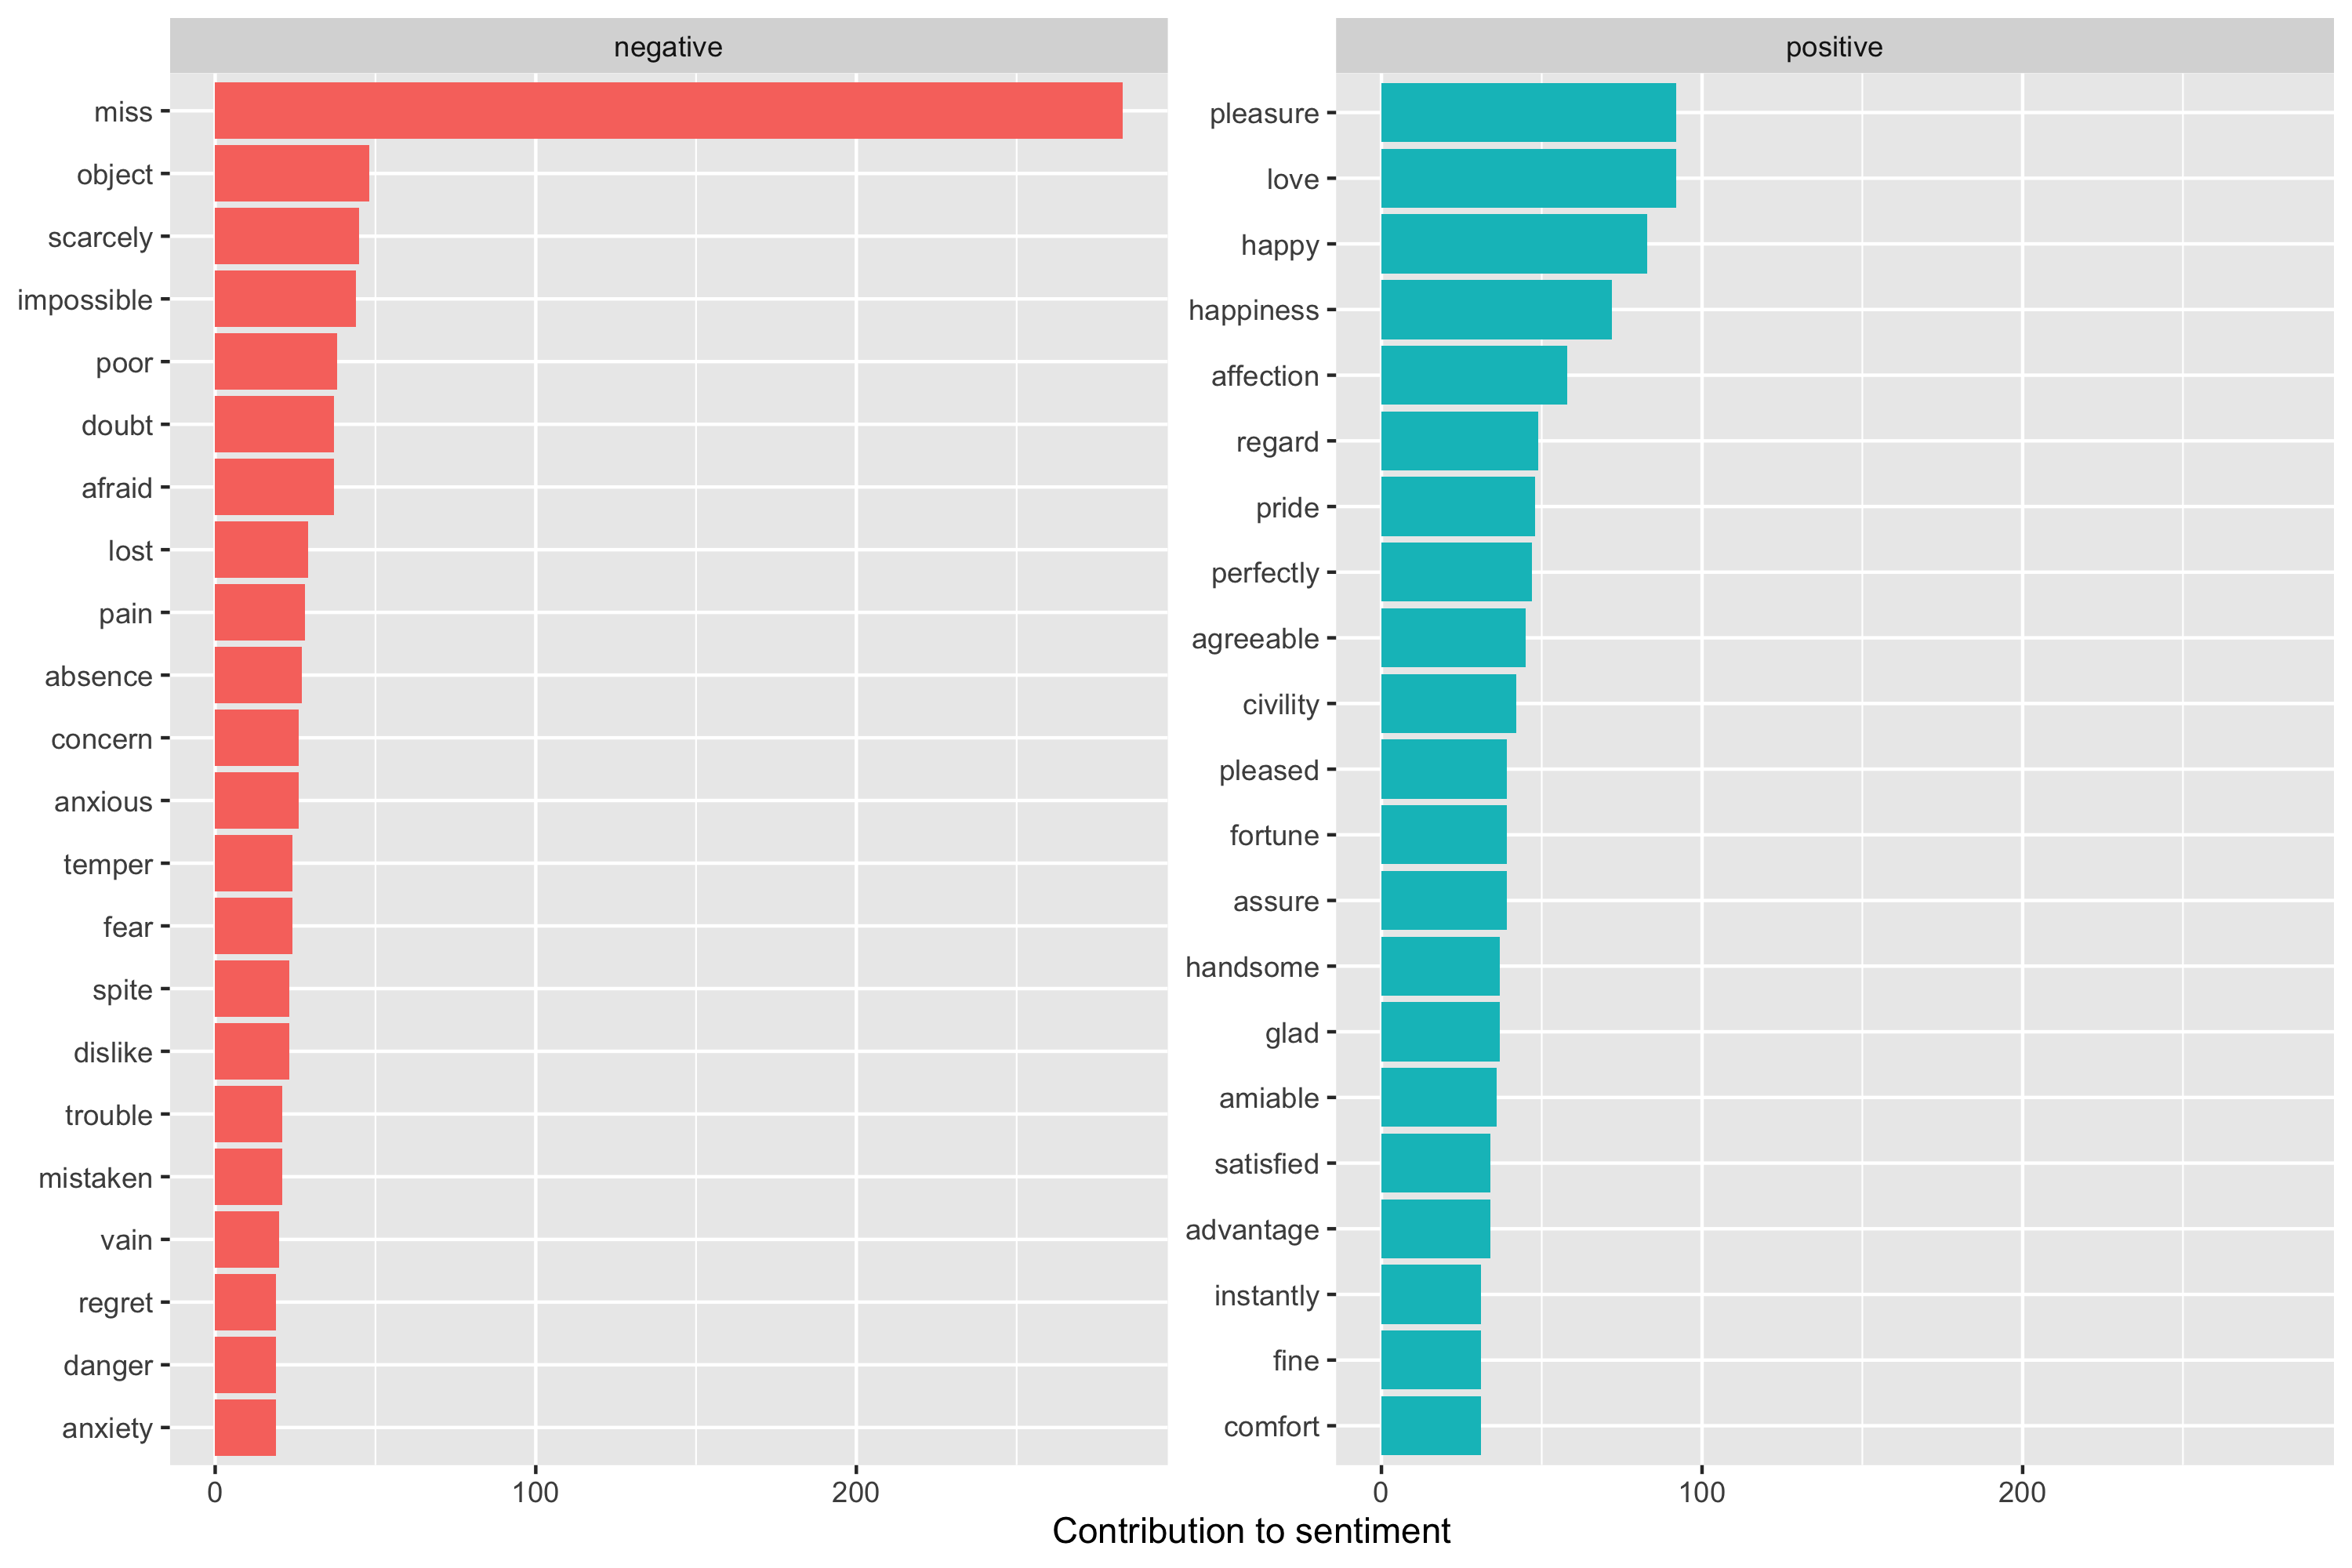
\includegraphics[width=1\linewidth]{Sentiment_austen.png}  
  \caption{Pride and Prejudice}
  \label{subfig2-1}
\end{subfigure}
\newline
\begin{subfigure}{1\textwidth}
  \centering
  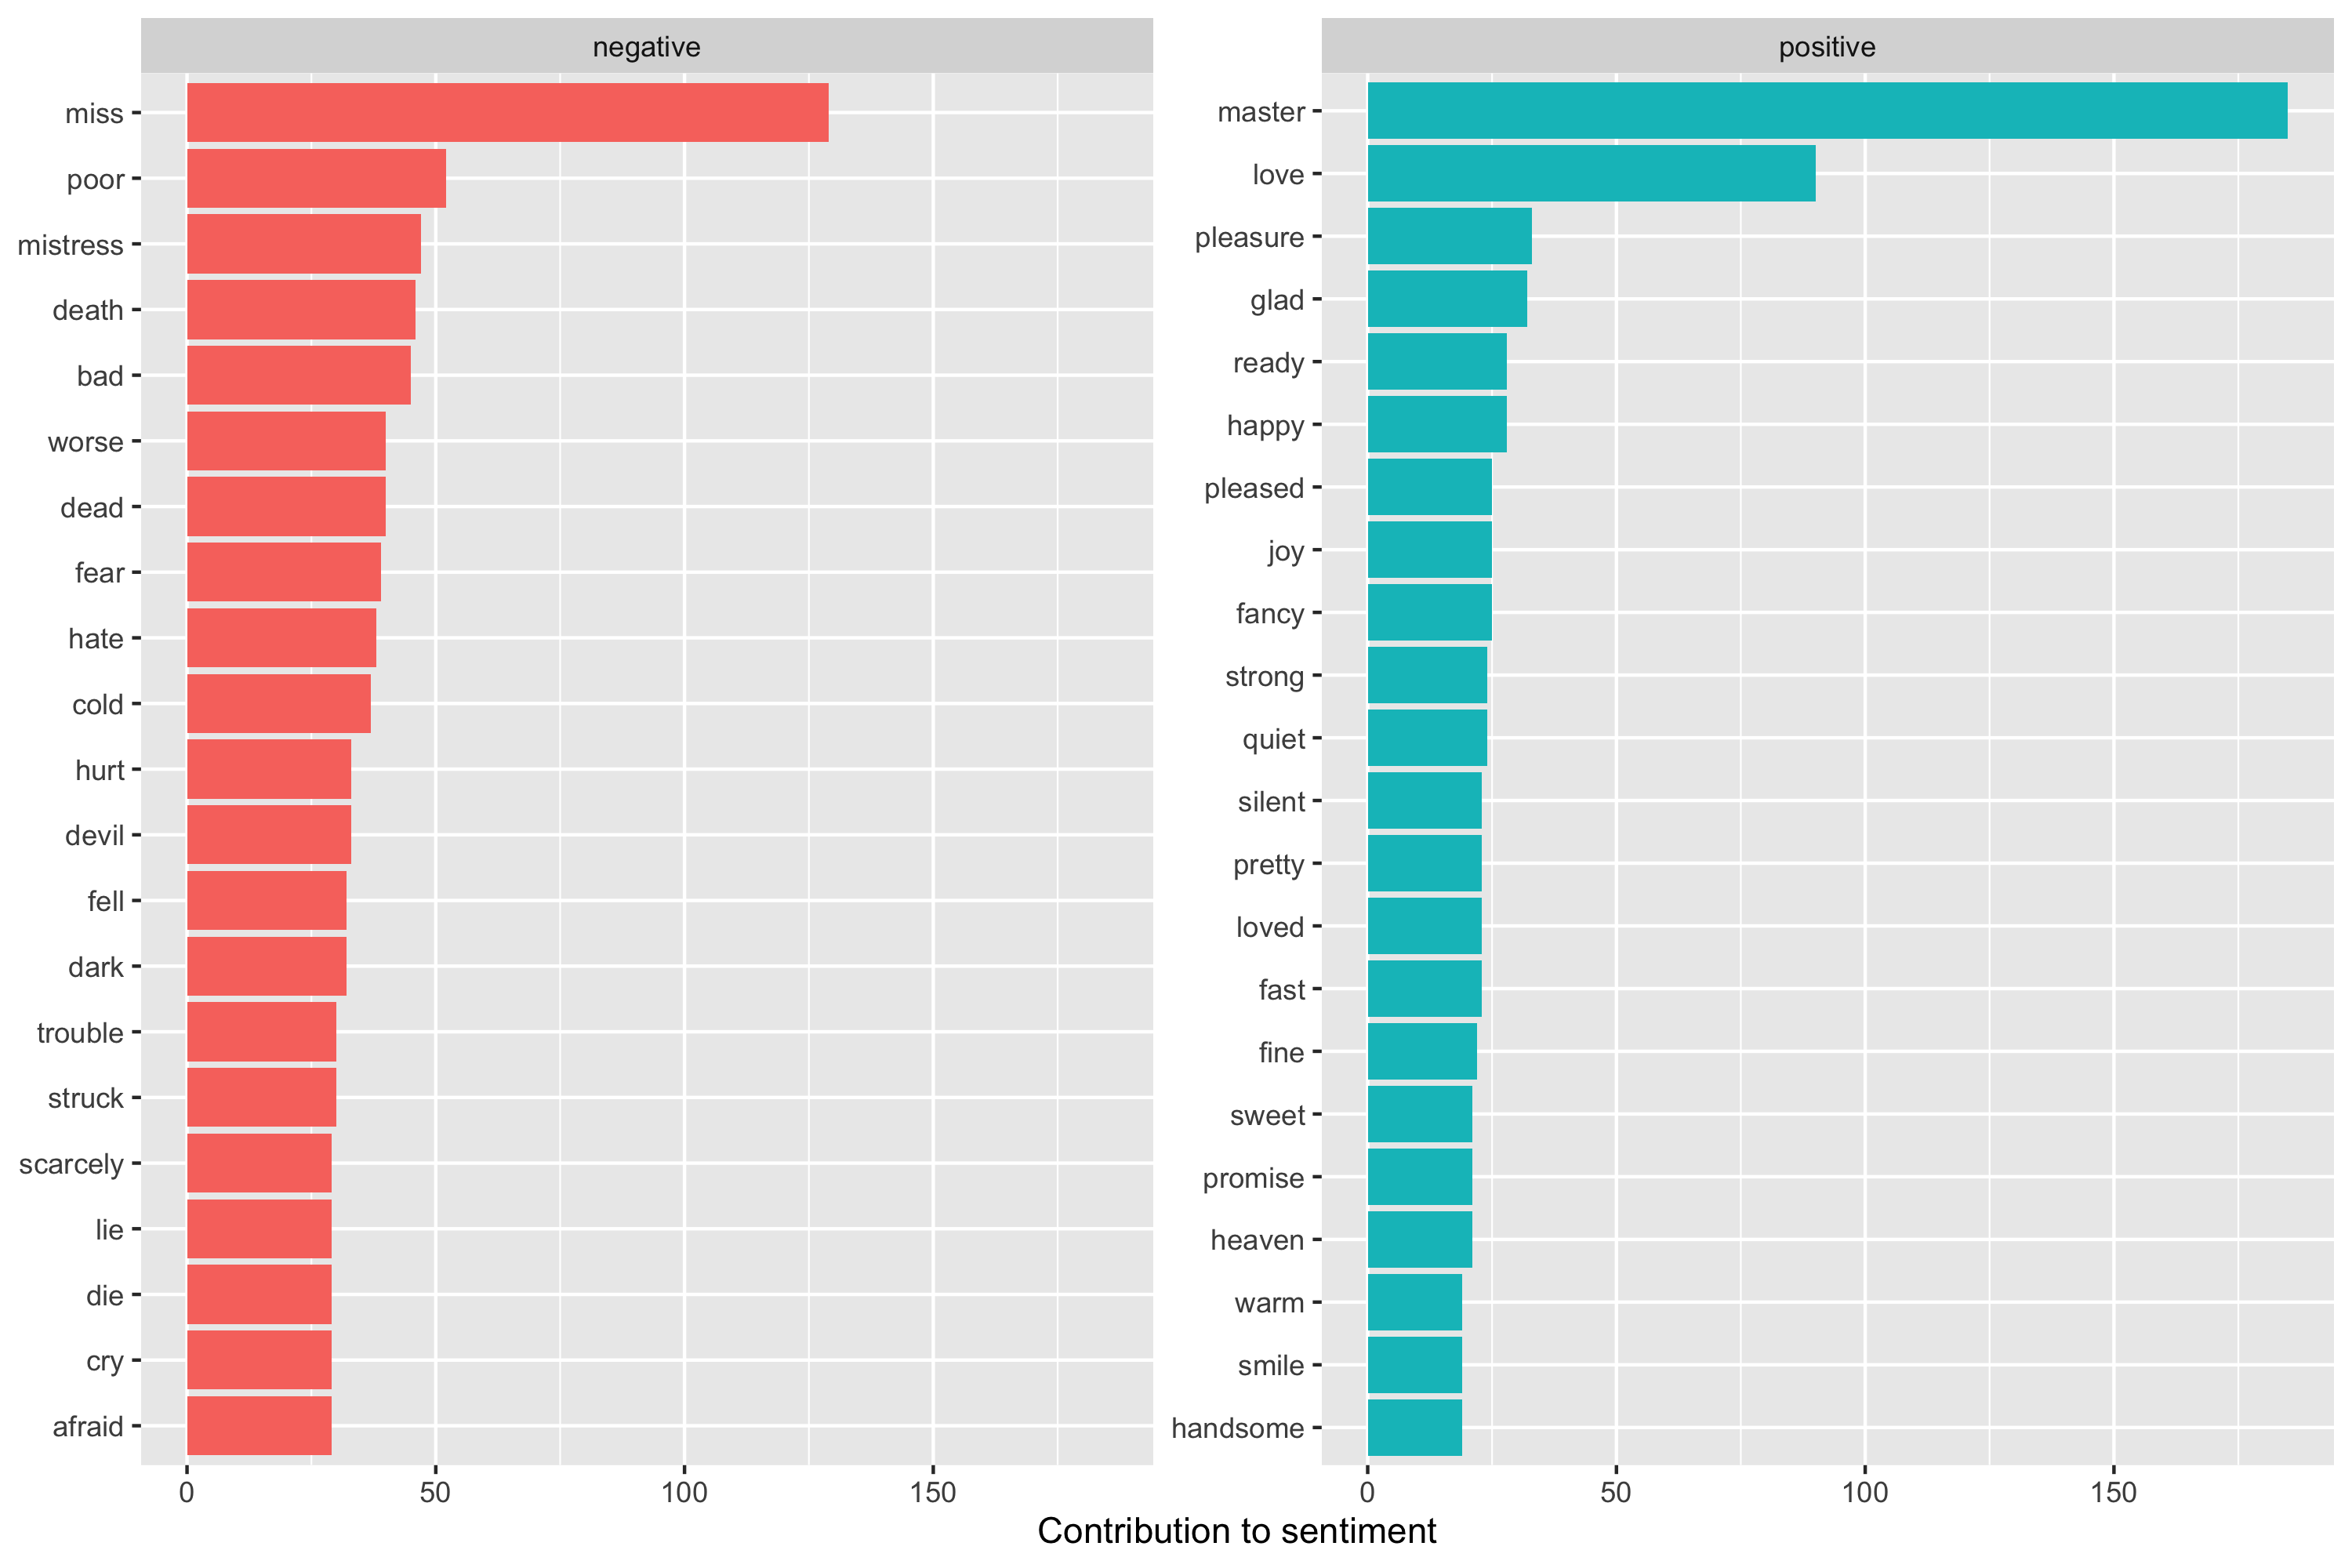
\includegraphics[width=1\linewidth]{Sentiment_bronte.png}  
  \caption{Wuthering Heights}
  \label{subfig2-2}
\end{subfigure}
\caption{Sentiment analysis of both books.}
\label{fig2}
\end{figure}

\clearpage

Having this outline of the sentiment analysis, we need to transform the data we have into something we can use for the histograms for the second part of this work. The reason we used the library \texttt{bing} for the sentiment analysis is because it divides the words into positive and negative emotions. With this, we transform them into binary data. \\

The first thing to know after this transformation is the distribution of positive versus negative words in both works. In Figure \ref{fig3} we used histograms to represent that distribution. If we add the positive and negative words in each book, we find that the difference between total of words is not that great. \textit{Pride and Prejudice} holds 7,523 words, while \textit{Wuthering Heights} has 7,976.\\

The main and visible difference is that in Subfigure \ref{subfig3-1} the positive and negative words are almost even, with positive words being slightly higher. In the case of Subfigure \ref{subfig3-2} we see a stark difference, being that the negative words represent almost two thirds of the total of words. \\


\begin{figure}[]
\begin{subfigure}{.5\textwidth}
  \centering
  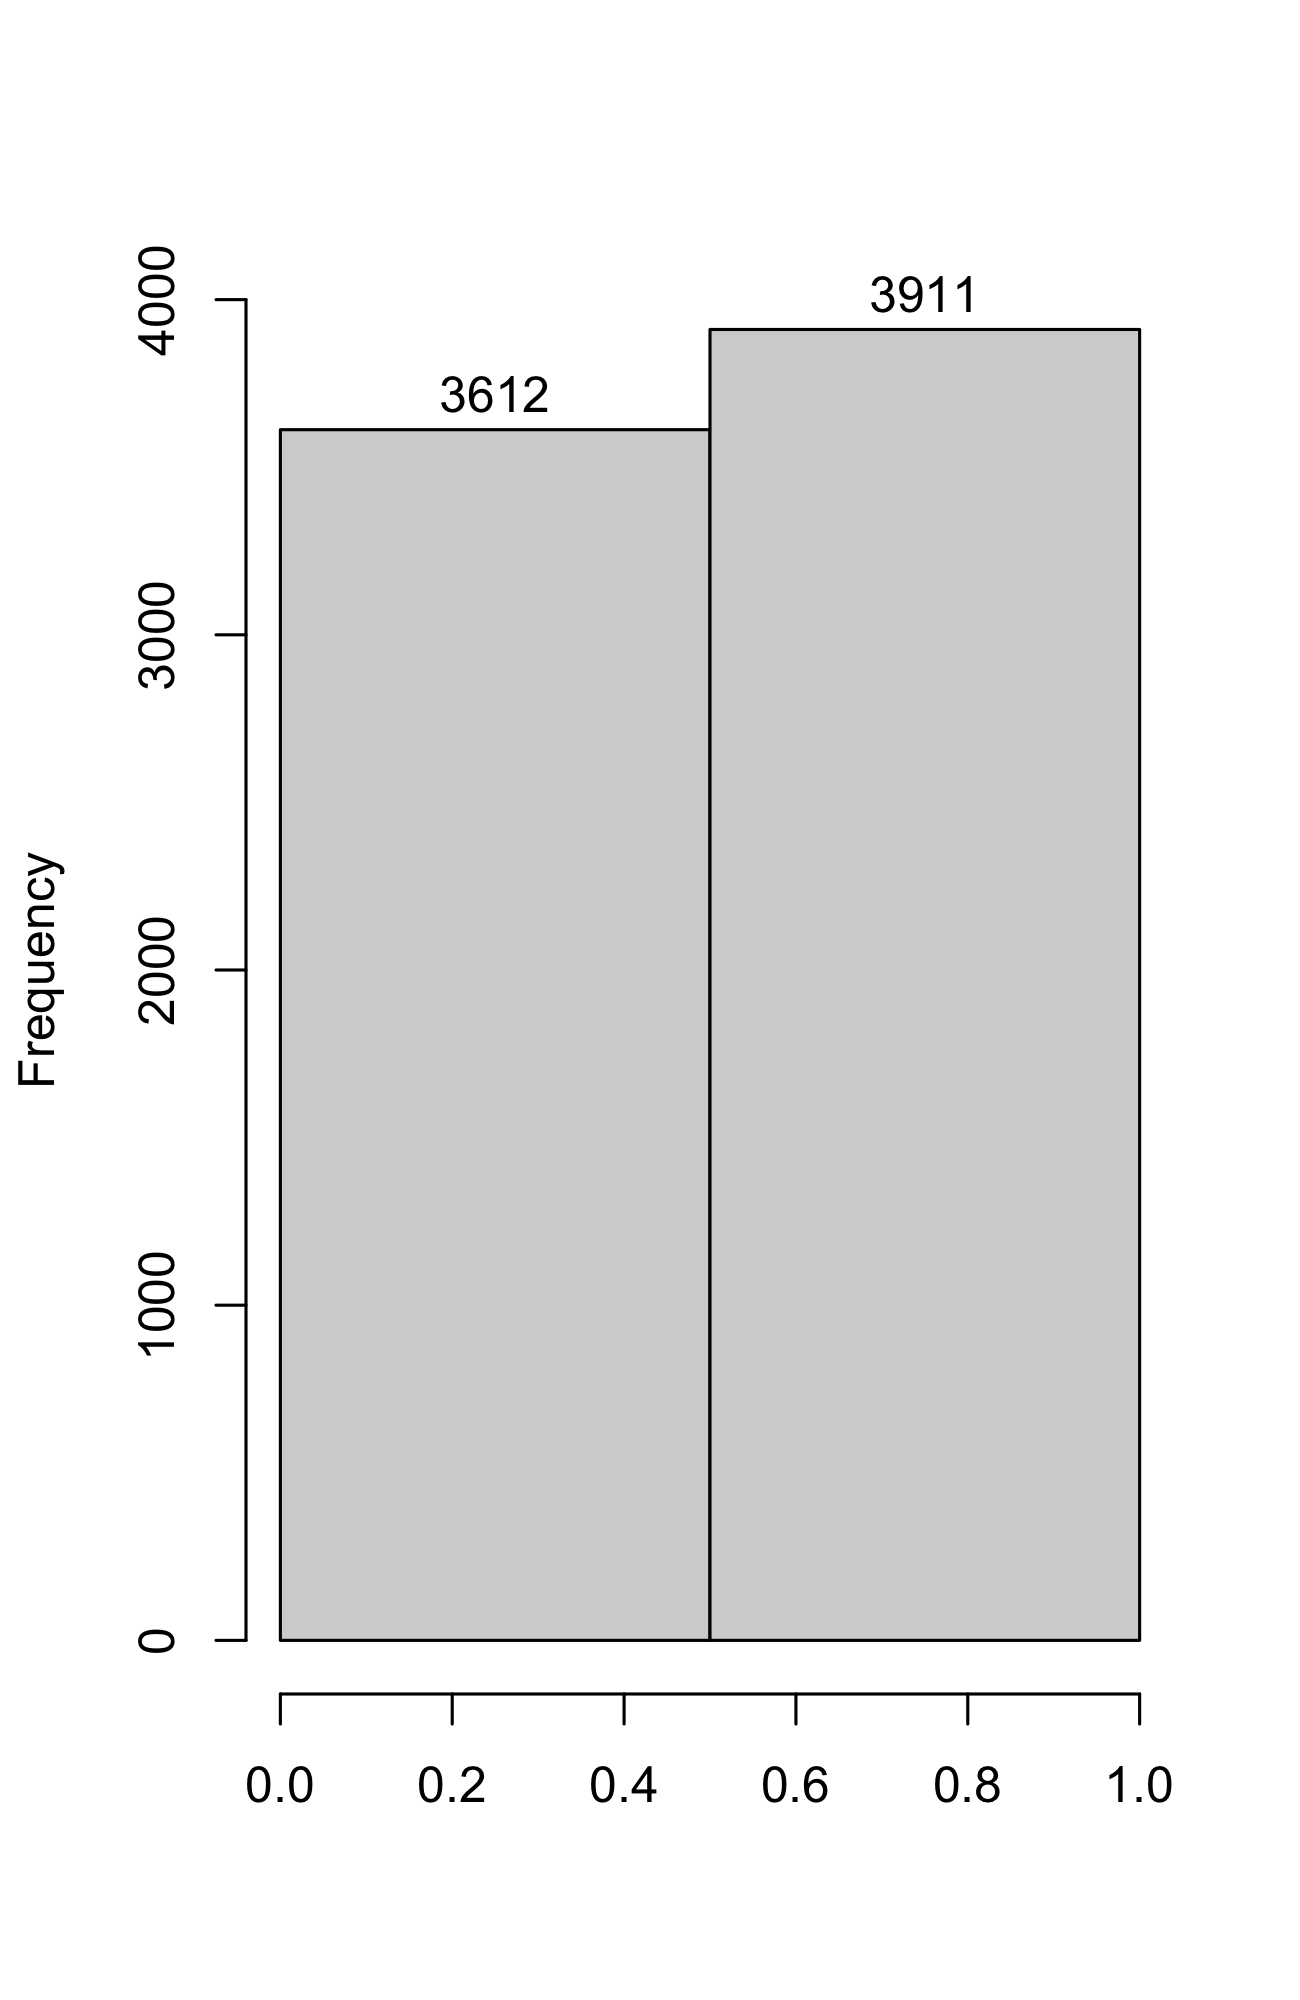
\includegraphics[width=1\linewidth]{posneg_austen.png}  
  \caption{Pride and Prejudice}
  \label{subfig3-1}
\end{subfigure}
\begin{subfigure}{.5\textwidth}
  \centering
  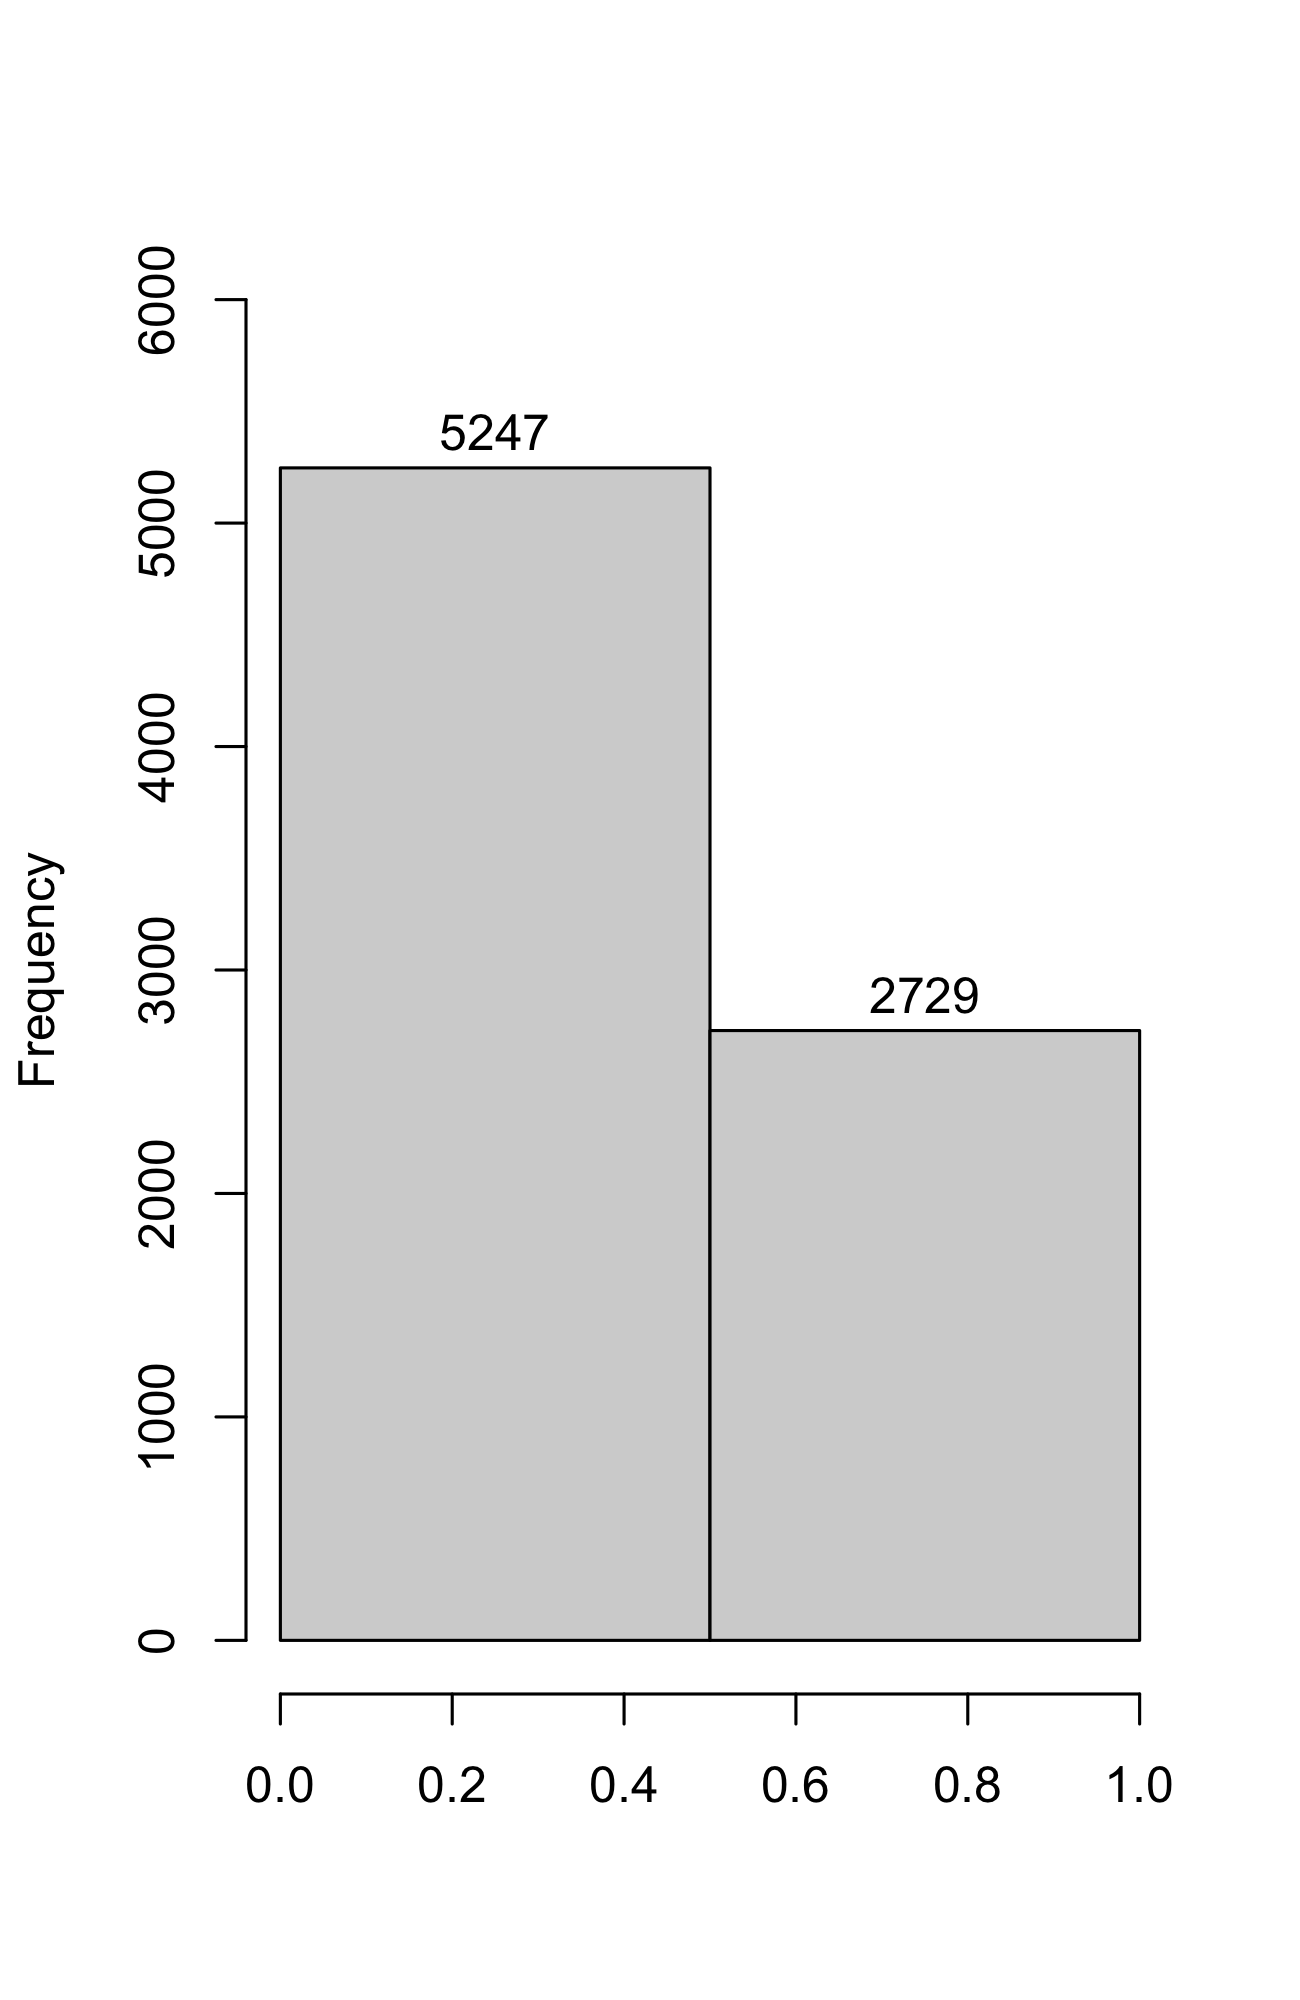
\includegraphics[width=1\linewidth]{posneg_bronte.png}  
  \caption{Wuthering Heights}
  \label{subfig3-2}
\end{subfigure}
\caption{Frequency of positive and negative words. Negative are represented in 0 and positive in 1.}
\label{fig3}
\end{figure}

In this case, Figure \ref{fig3} goes appropriately with the previous knowledge of the books. While both authors are female, lived in the 19th century and both are novelists, the feeling of the book is quite different. While in \textit{Pride and Prejudice} our main protagonist Elizabeth is guilty of being biased and proud in her view of Darcy, and he in turn was spoiled and prideful as well, they are quite tamed compared with how volatile and prone to violence Heathcliff is. Also, the main protagonist Catherine is very selfish and cruel to everyone around her. \\

For this, the difference in characters behaviour, can be interpreted as one of the main reasons for the disparity in distribution of positive and negative words.\\
 
%\clearpage

\begin{figure}[]
\begin{subfigure}{.5\textwidth}
  \centering
  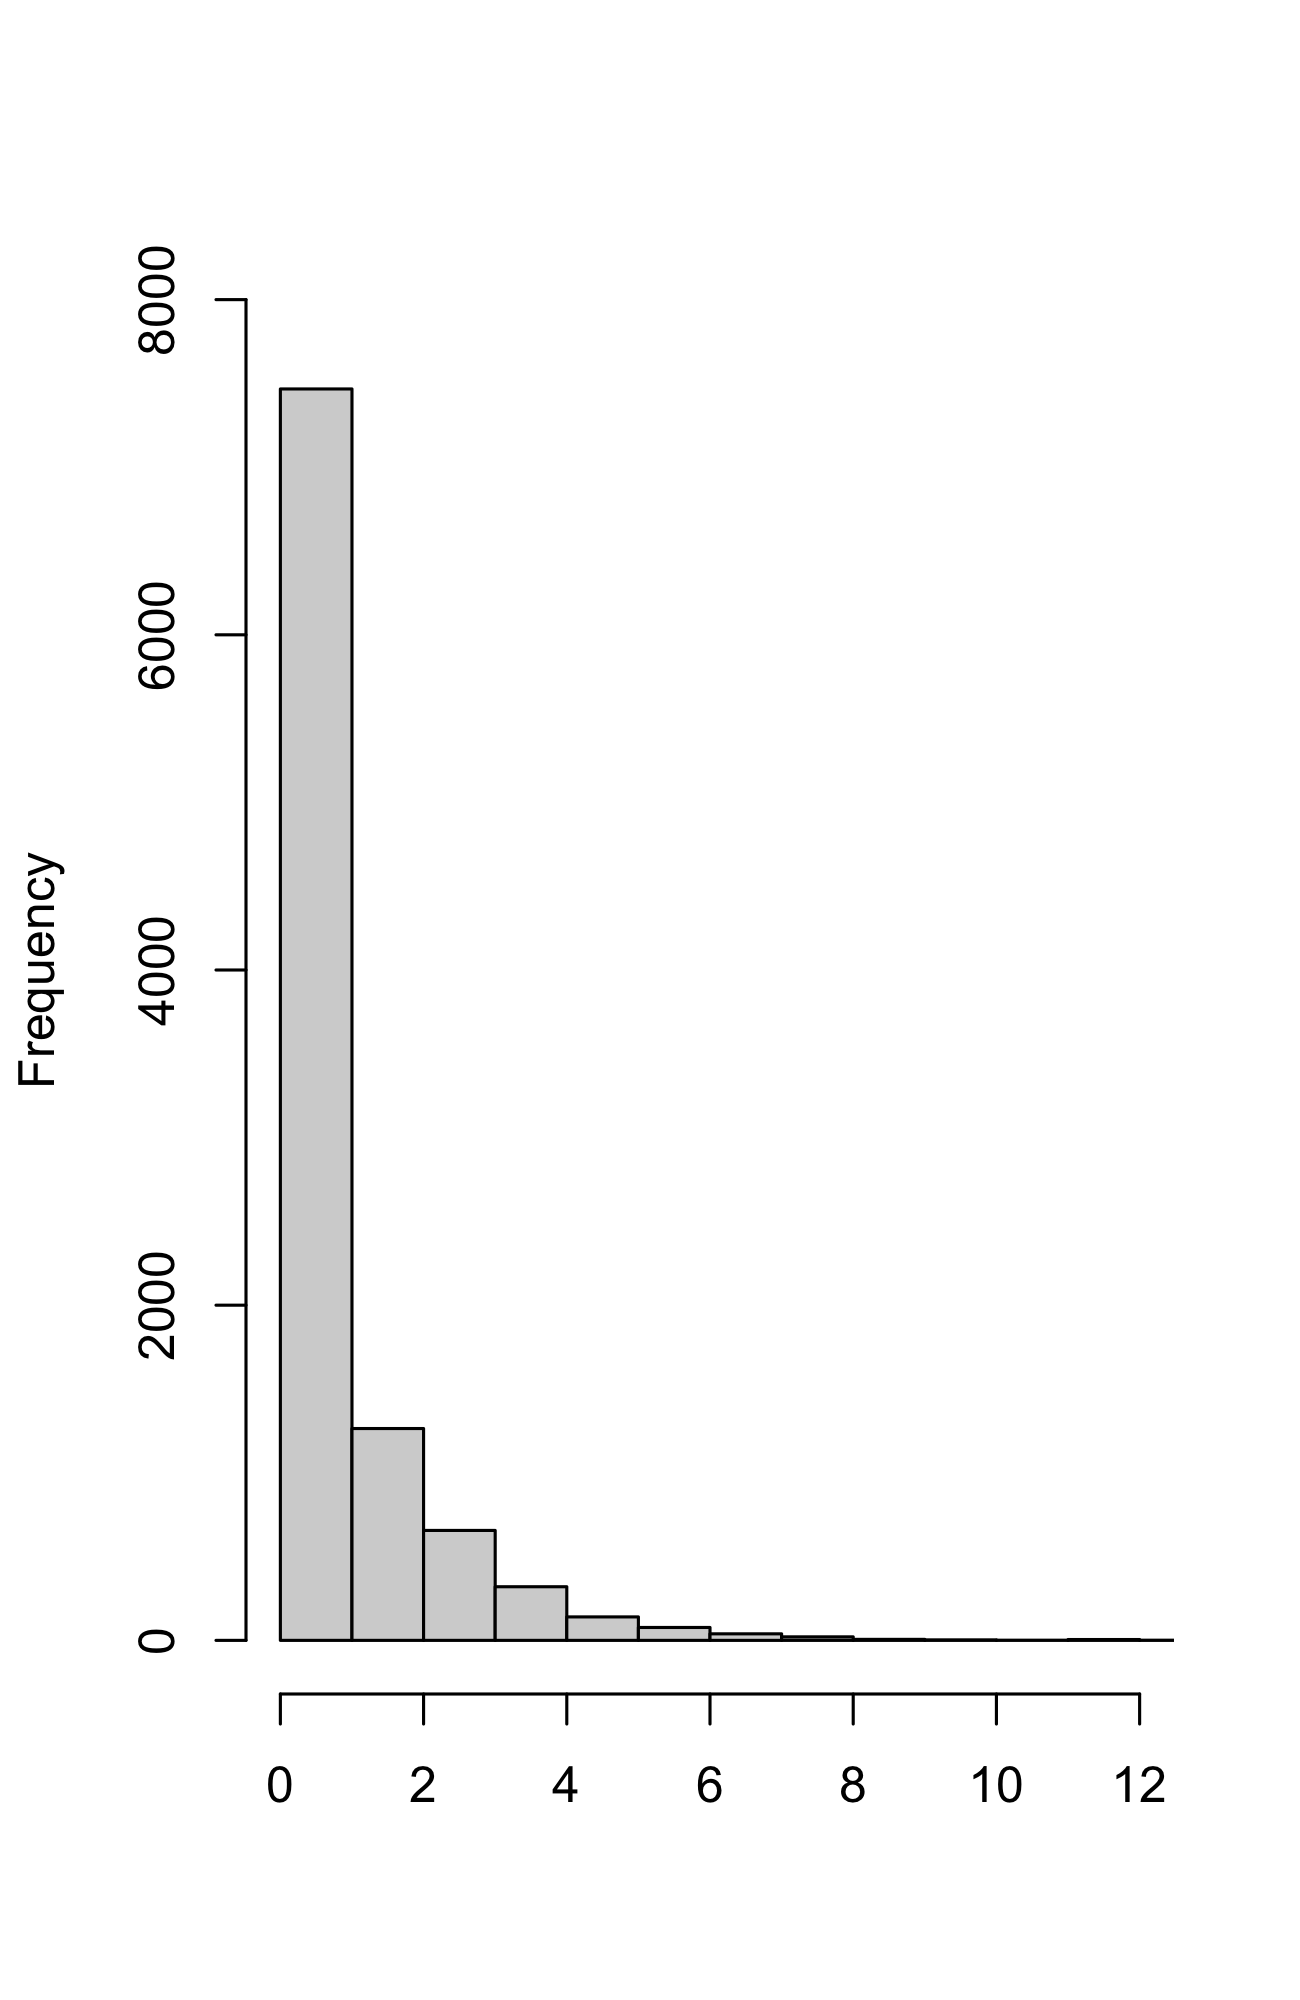
\includegraphics[width=1\linewidth]{rgeom_austen.png}  
  \caption{Histogram with rgeom tool.}
  \label{subfig4-1}
\end{subfigure}
\begin{subfigure}{.5\textwidth}
  \centering
  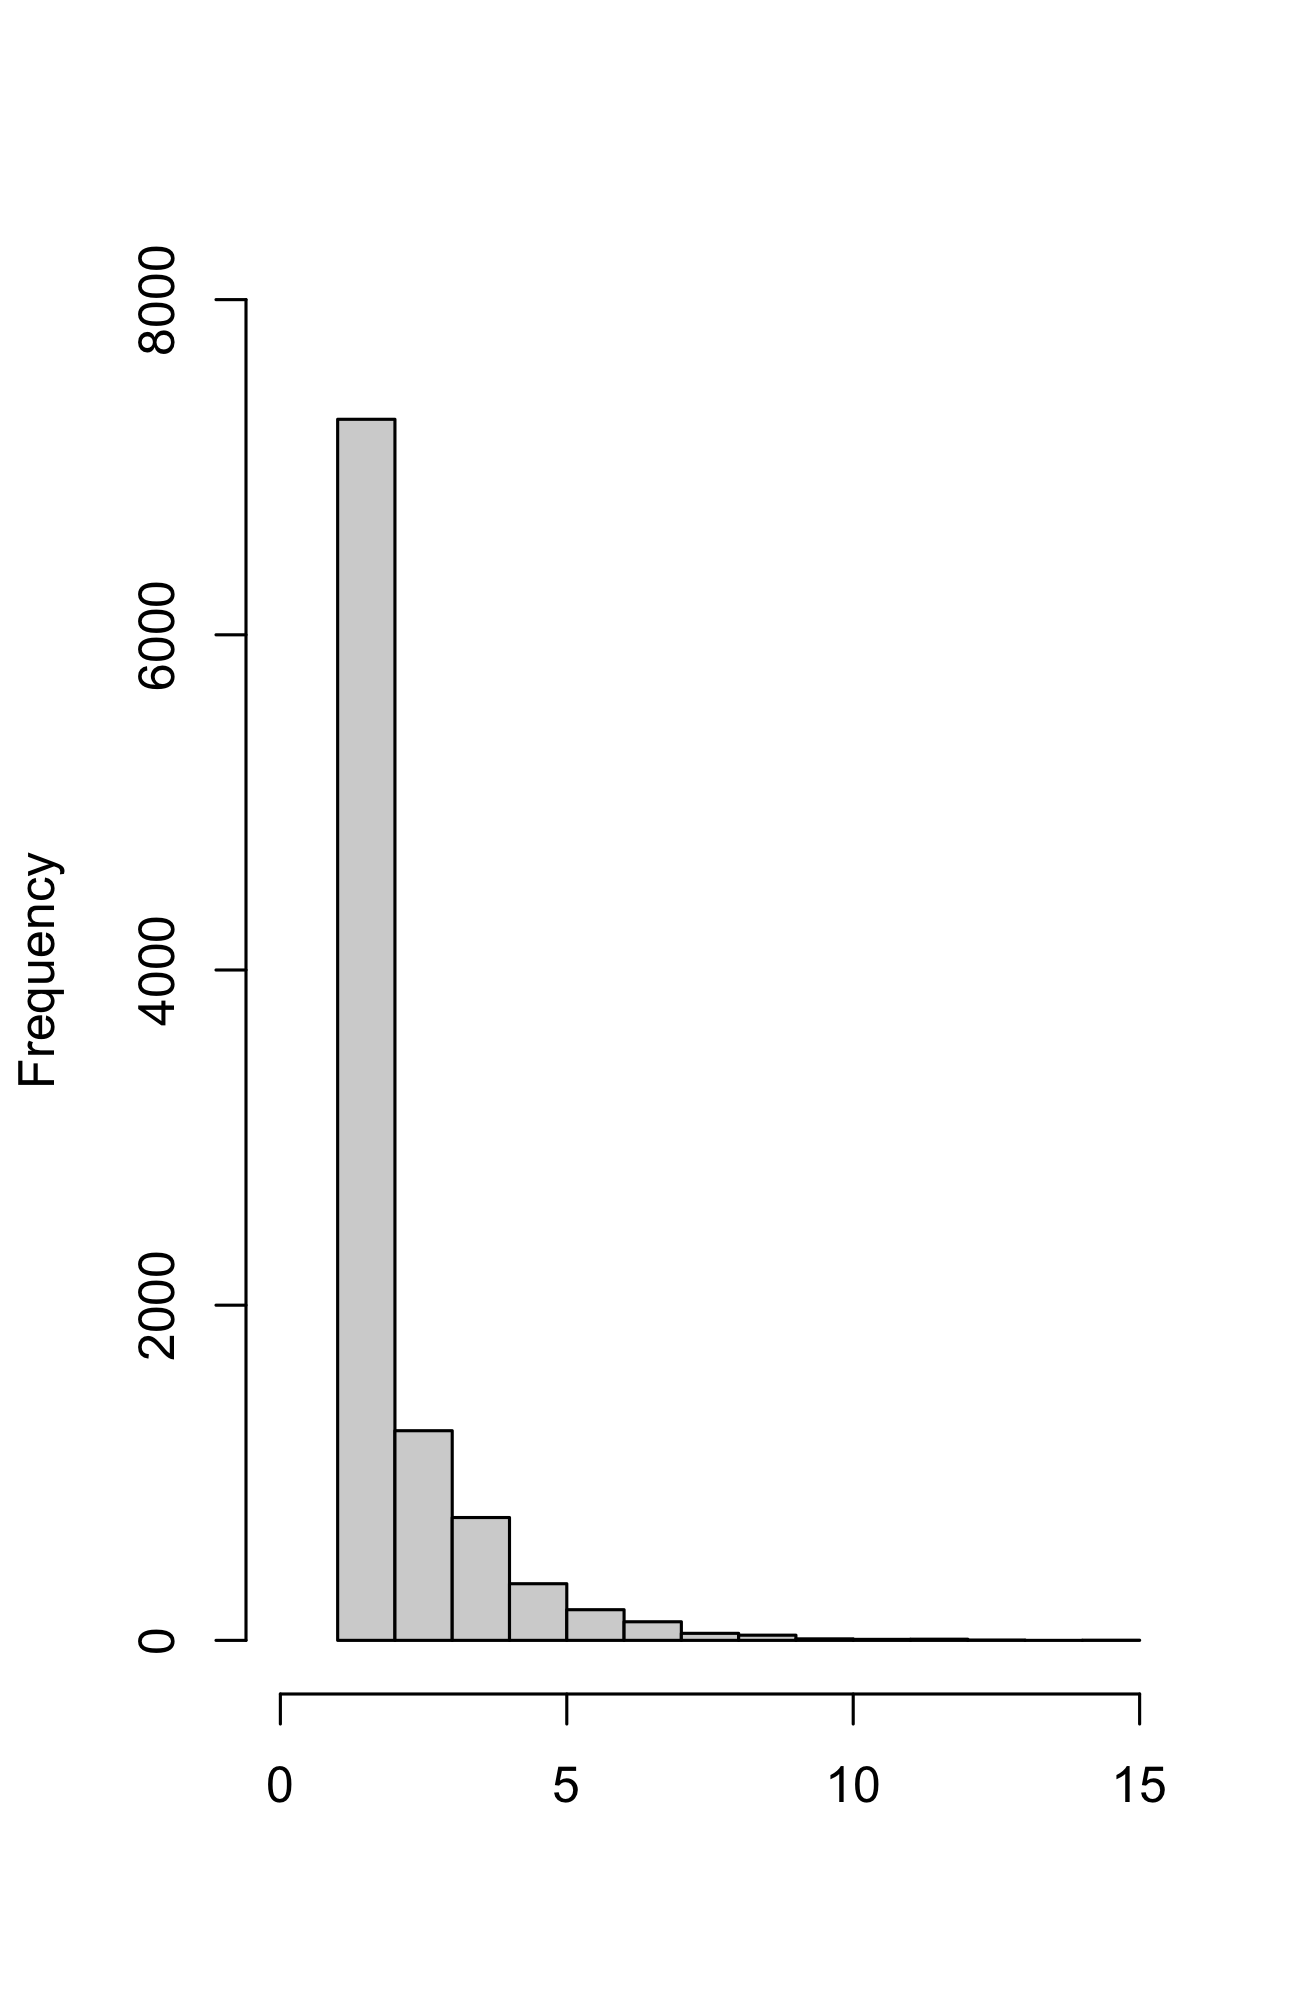
\includegraphics[width=1\linewidth]{co_rgeom_austen.png}  
  \caption{Histogram with made code.}
  \label{subfig4-2}
\end{subfigure}
\caption{Comparison between the use of the tool \texttt{rgeom} and a made code on the book Pride and Prejudice.}
\label{fig4}
\end{figure}

Having confirmed our first idea of the difference in tone in the books, we now use the information of the positive and negative words to perform distribution experiments. In Figure \ref{fig4} we first perform an experiment with the tool \texttt{rgeom} \cite{rgeom} with the same variables we have in our data, to see if we can recreate something similar with our interpretation of the problem in a made code. \\

The \texttt{rgeom} tool takes a number of experiments and the percentage of success we have. In both cases we take as success if they have a positive word, so the percentage we give is the ones we calculated from our data. In the case of \textit{Pride and Prejudice}, we have a percentage of 51\% positive words, and in \textit{Wuthering Heights} we have a 34\%. \\

In Subfigure \ref{subfig4-1} we have the result of a 10,000 repetition of the experiment with a 0.51 probability of success. We replicated the experiments using our data of binary information, and with the tool \texttt{sample} we take a \say{word} and we see if it is a success (positive) or not (negative). As we can see, the behaviour of both plots is almost the same. \\

%\clearpage

\begin{figure}[]
\begin{subfigure}{.5\textwidth}
  \centering
  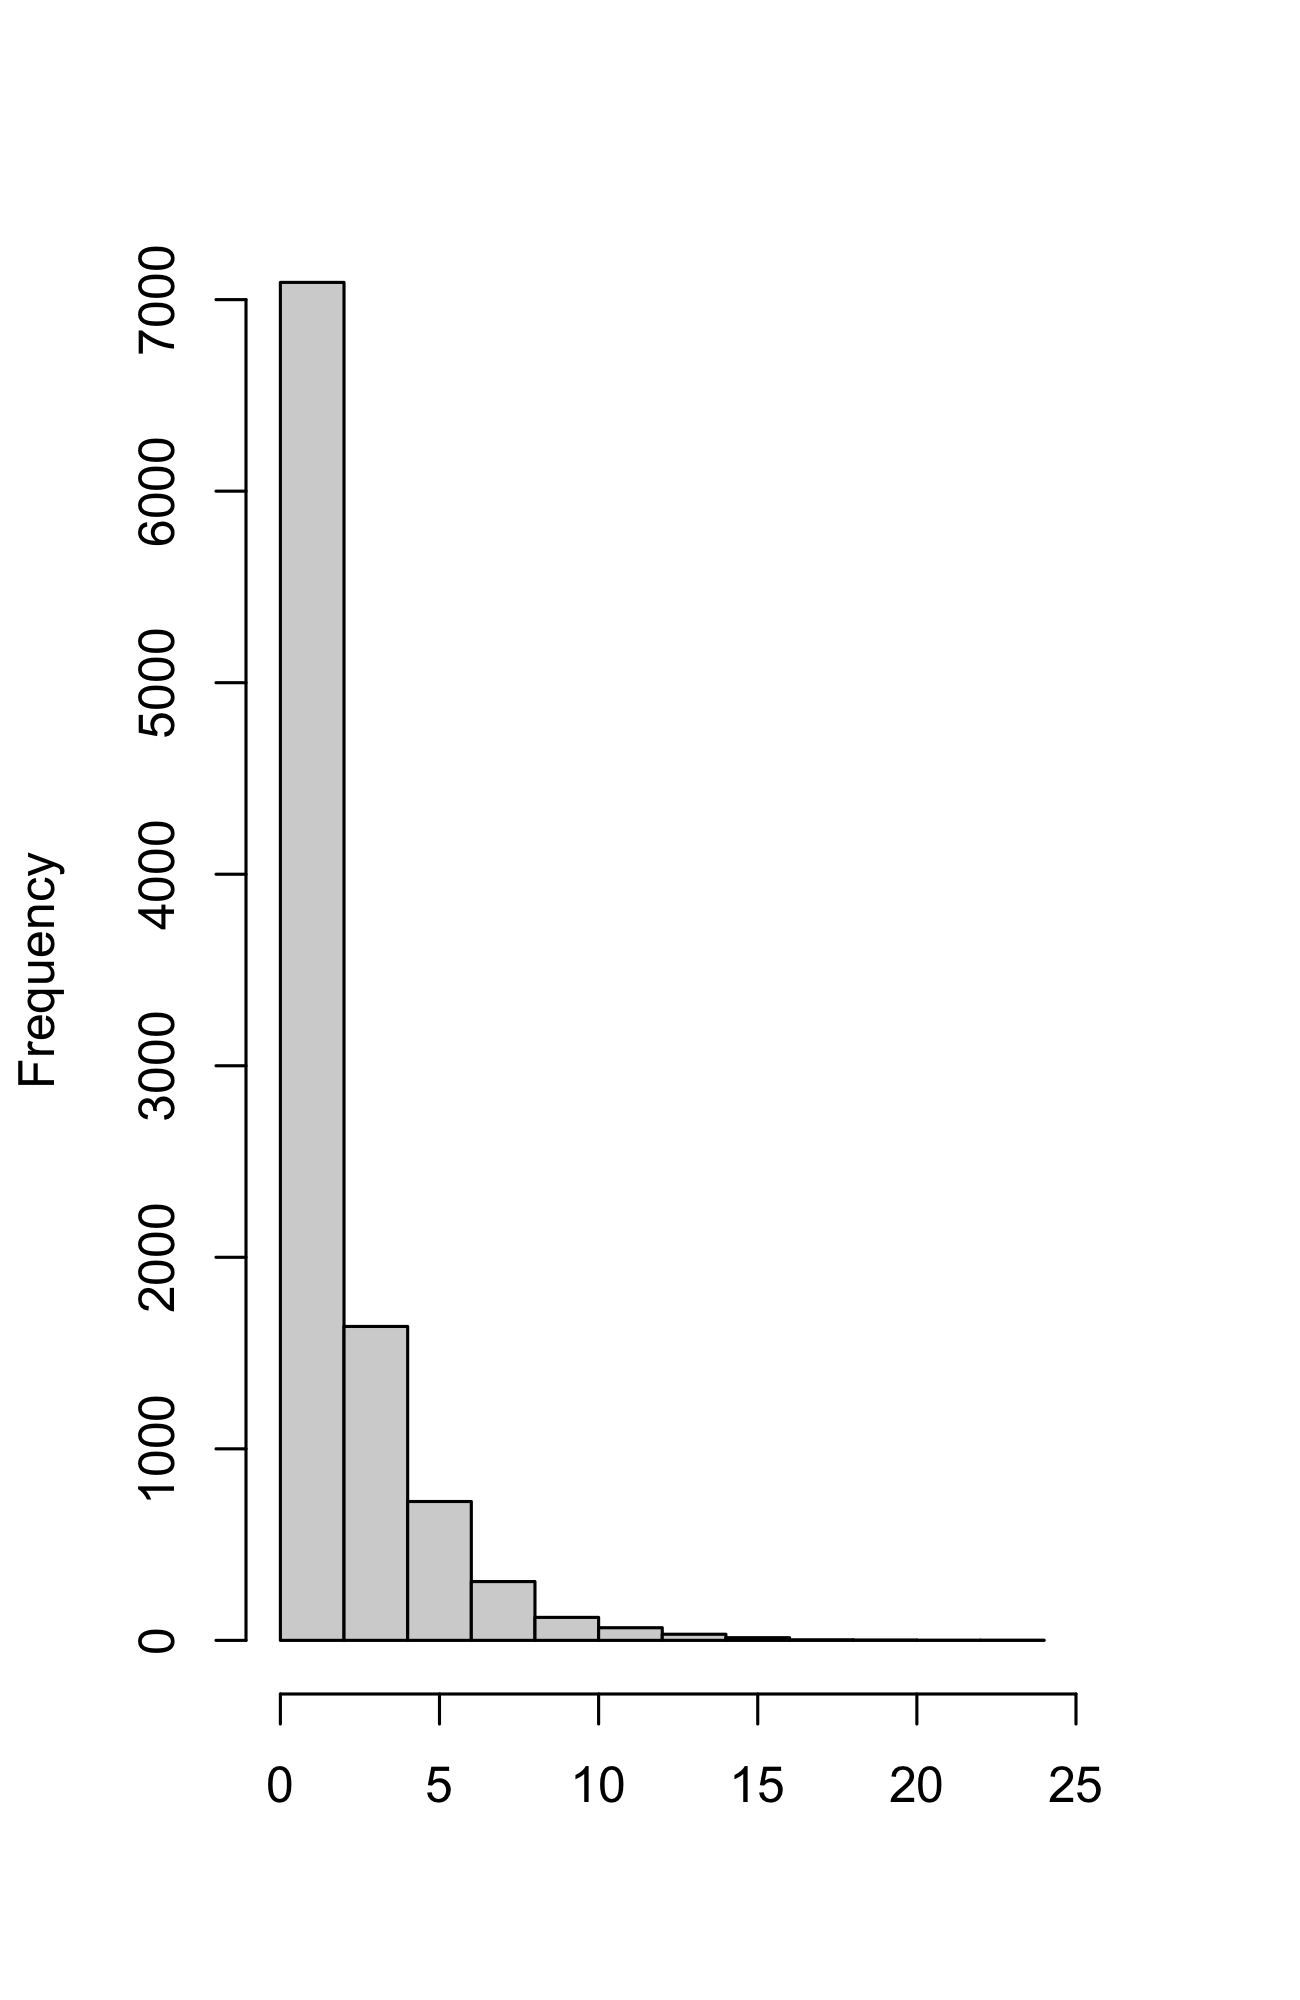
\includegraphics[width=1\linewidth]{rgeom_bronte.png}  
  \caption{Histogram with rgeom tool}
  \label{subfig5-1}
\end{subfigure}
\begin{subfigure}{.5\textwidth}
  \centering
  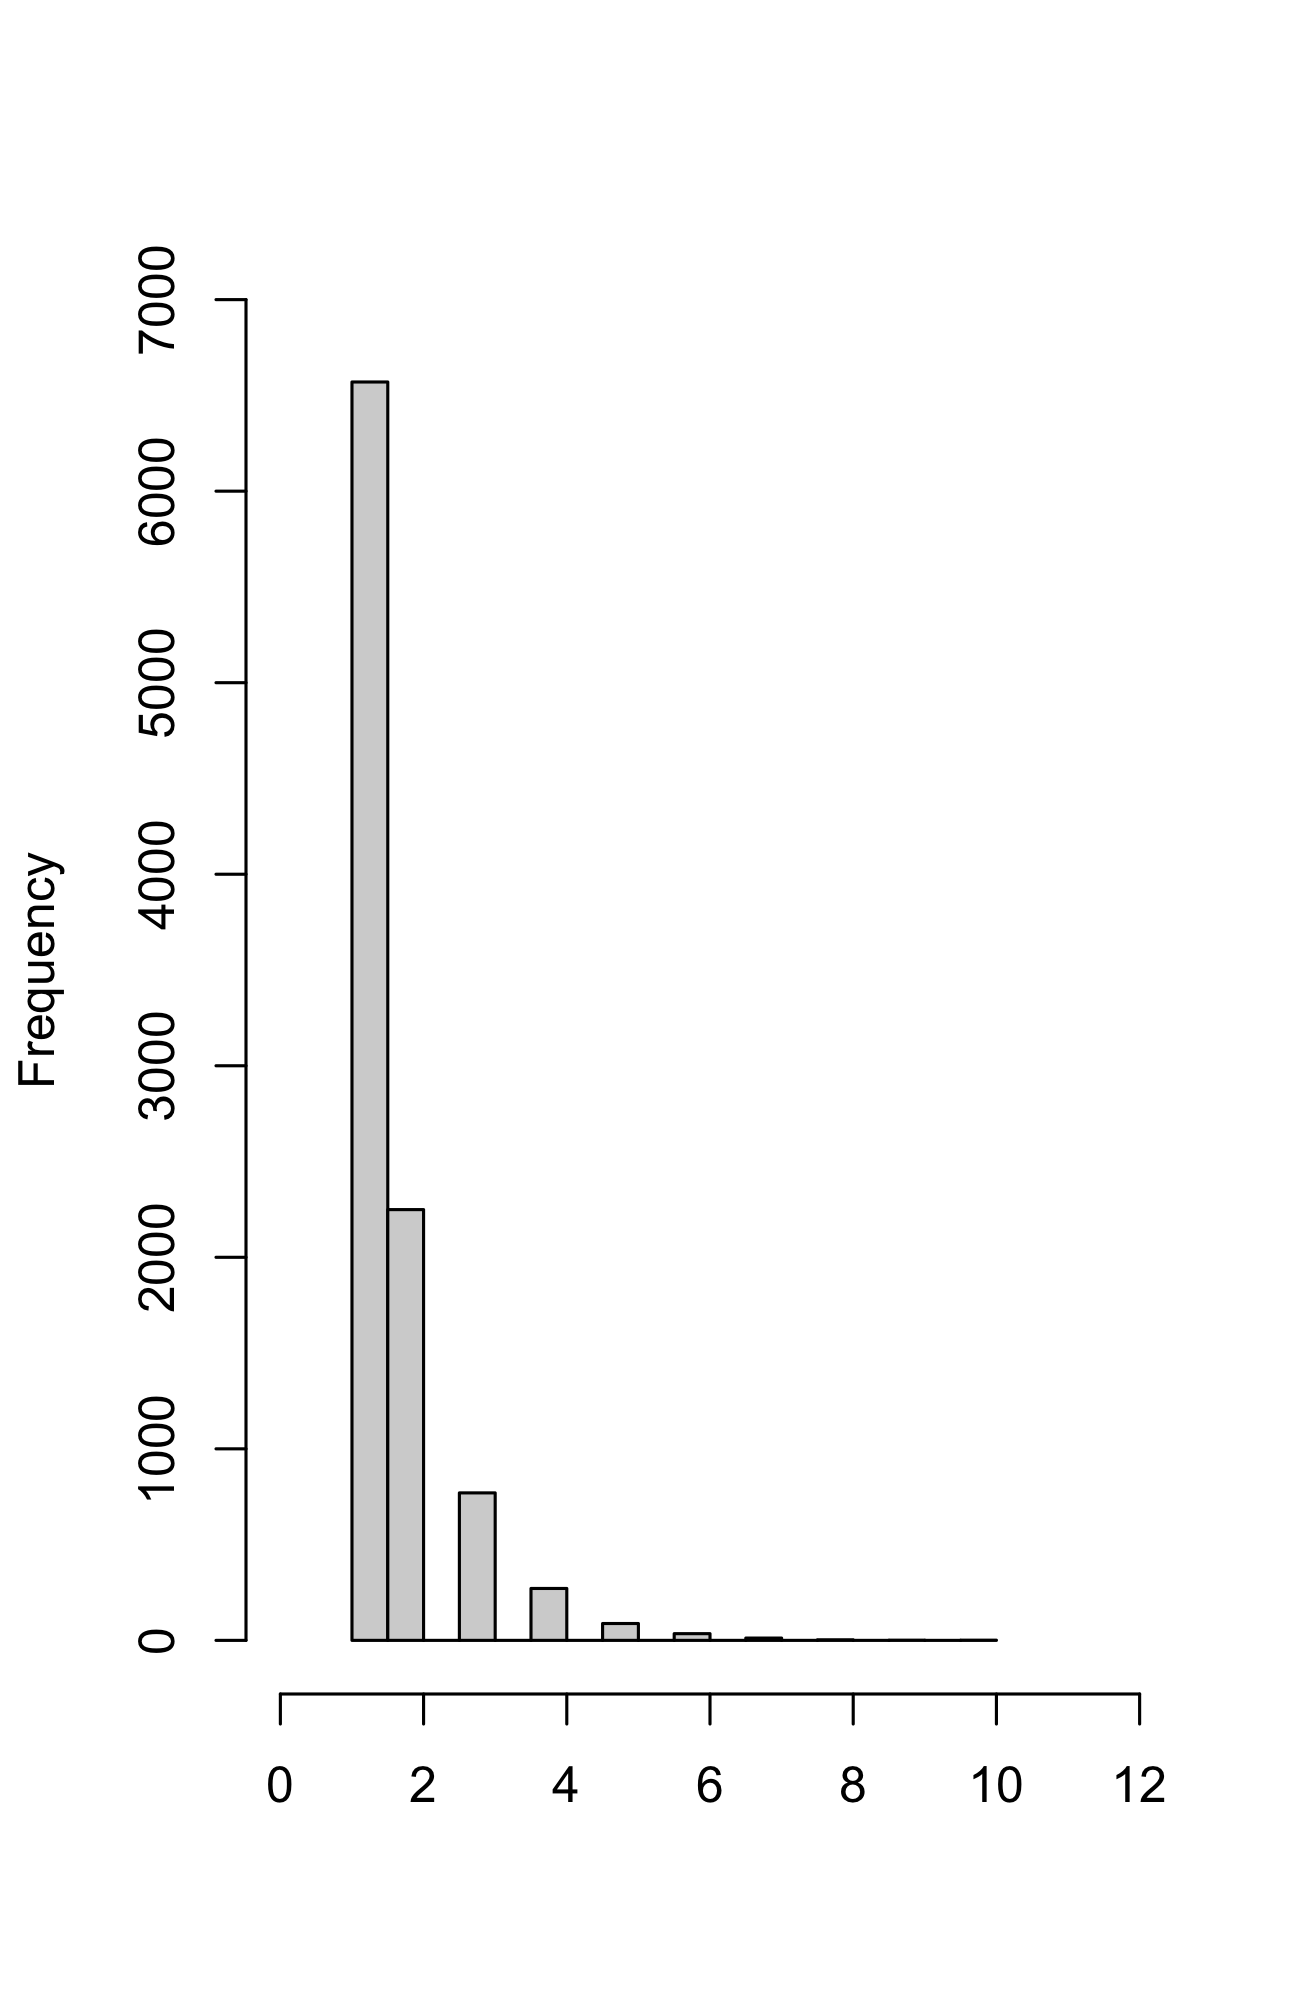
\includegraphics[width=1\linewidth]{co_rgeom_bronte.png}  
  \caption{Histogram with made code}
  \label{subfig5-2}
\end{subfigure}
\caption{Comparison between the use of the tool \texttt{rgeom} and a made code on the book Wuthering Heights}
\label{fig5}
\end{figure}


In Figure \ref{fig5} we have the same experimentation, but with the book \textit{Wuthering Heights}. In this case the difference between the subfigures are a bit more noticeable than in the previous experiment. In Subfigure \ref{subfig5-1} we have the result of a 10,000 repetition of the experiment with a 0.34 probability of success. Subfigure \ref{subfig5-2} uses the same made code than in Subfigure \ref{subfig4-2} changing only the parameters of probability and the data used.\\
%\clearpage

\begin{figure}[]
\begin{subfigure}{.5\textwidth}
  \centering
  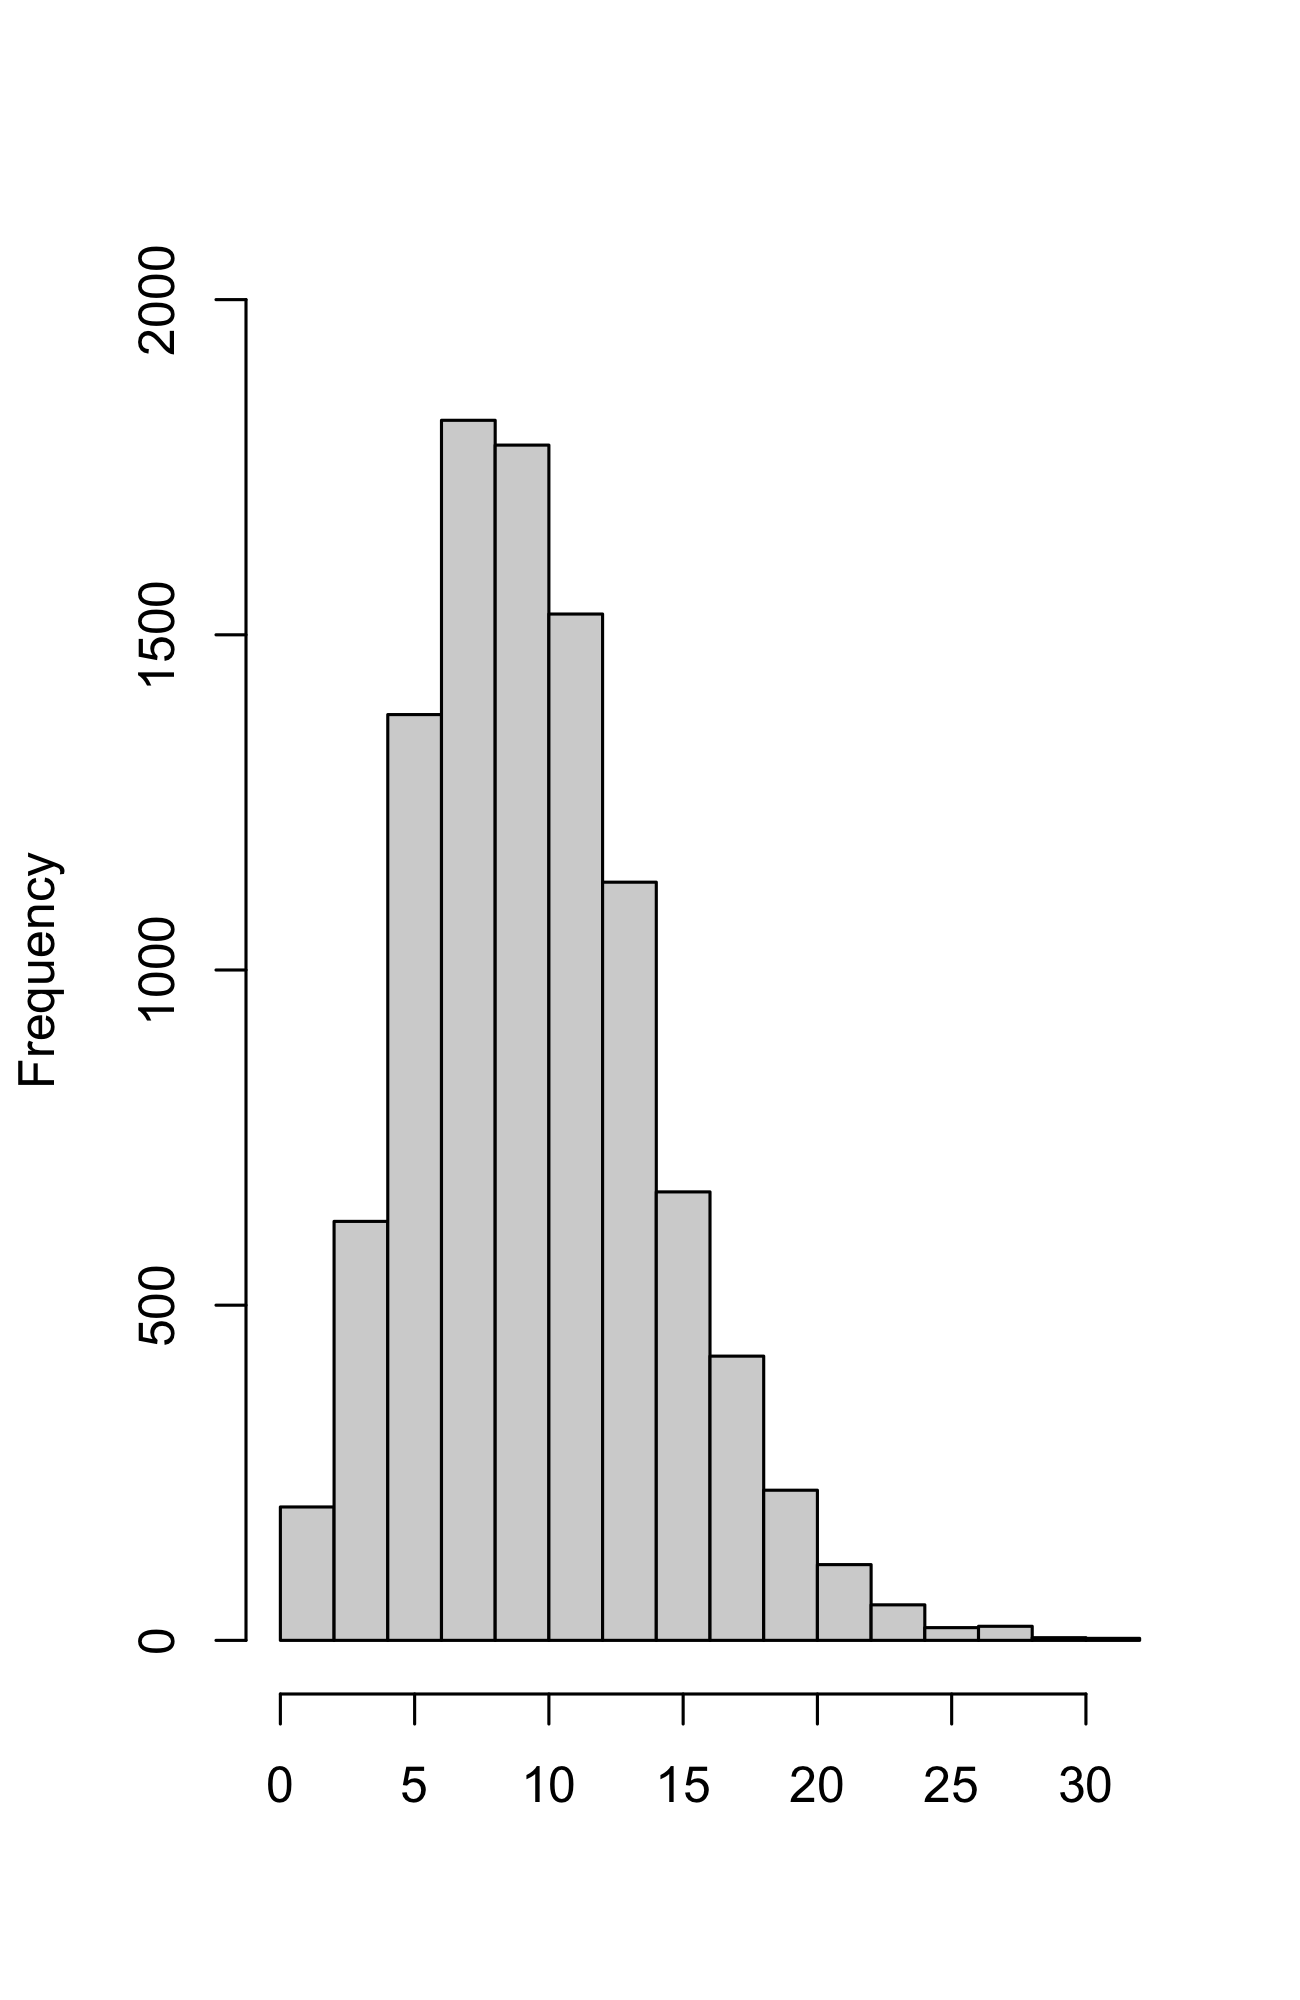
\includegraphics[width=.8\linewidth]{rbinom_austen.png}  
  \caption{Using rbinom, Pride and Prejudice.}
  \label{subfig6-1}
\end{subfigure}
\begin{subfigure}{.5\textwidth}
  \centering
  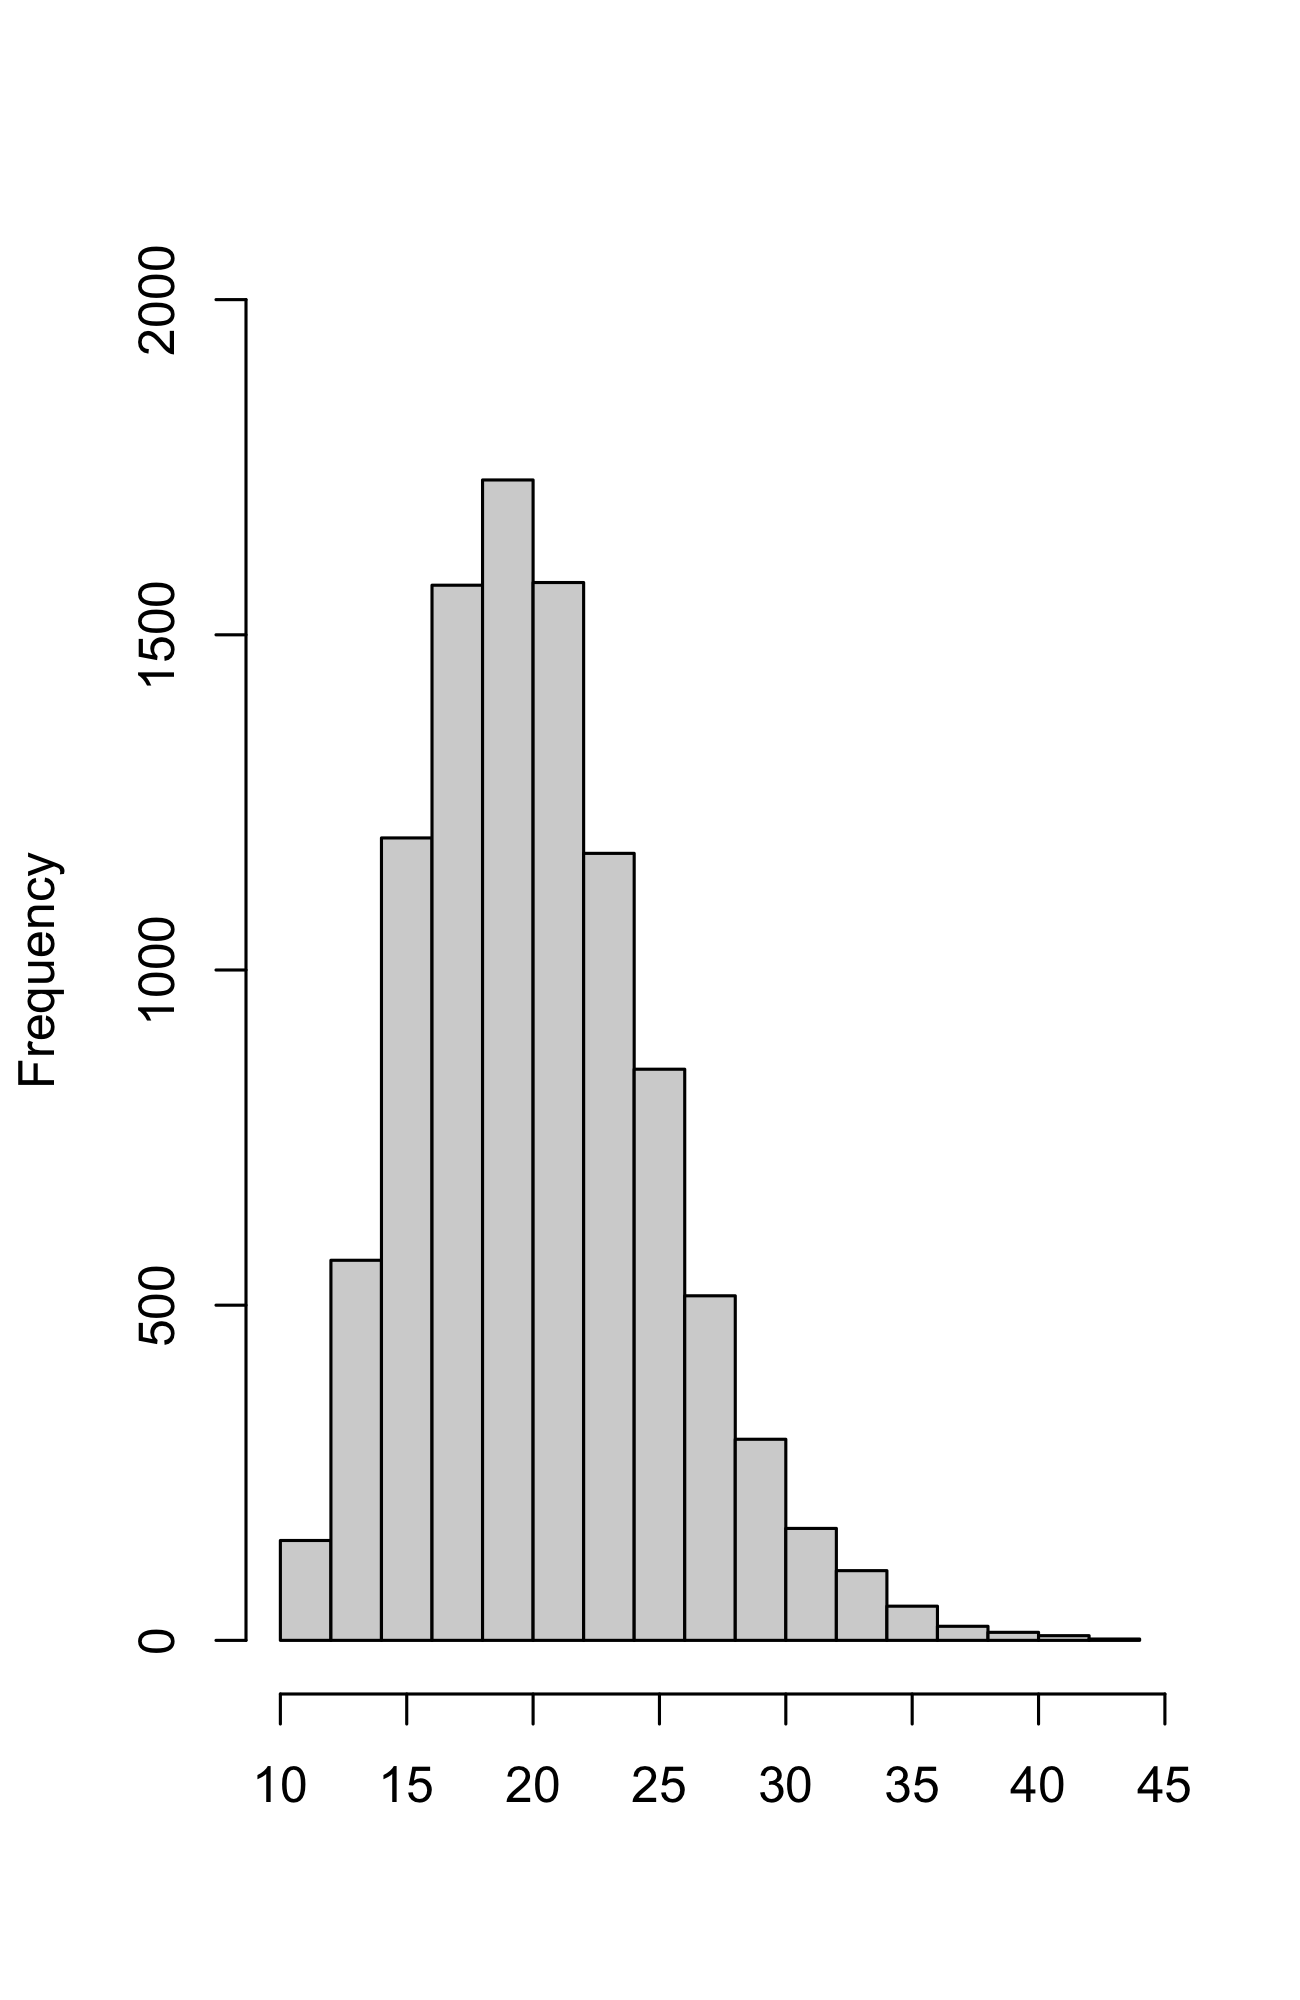
\includegraphics[width=.8\linewidth]{co_rbinom_austen.png}  
  \caption{Using made code, Pride and Prejudice.}
  \label{subfig6-2}
\end{subfigure}
\newline
\begin{subfigure}{.5\textwidth}
  \centering
  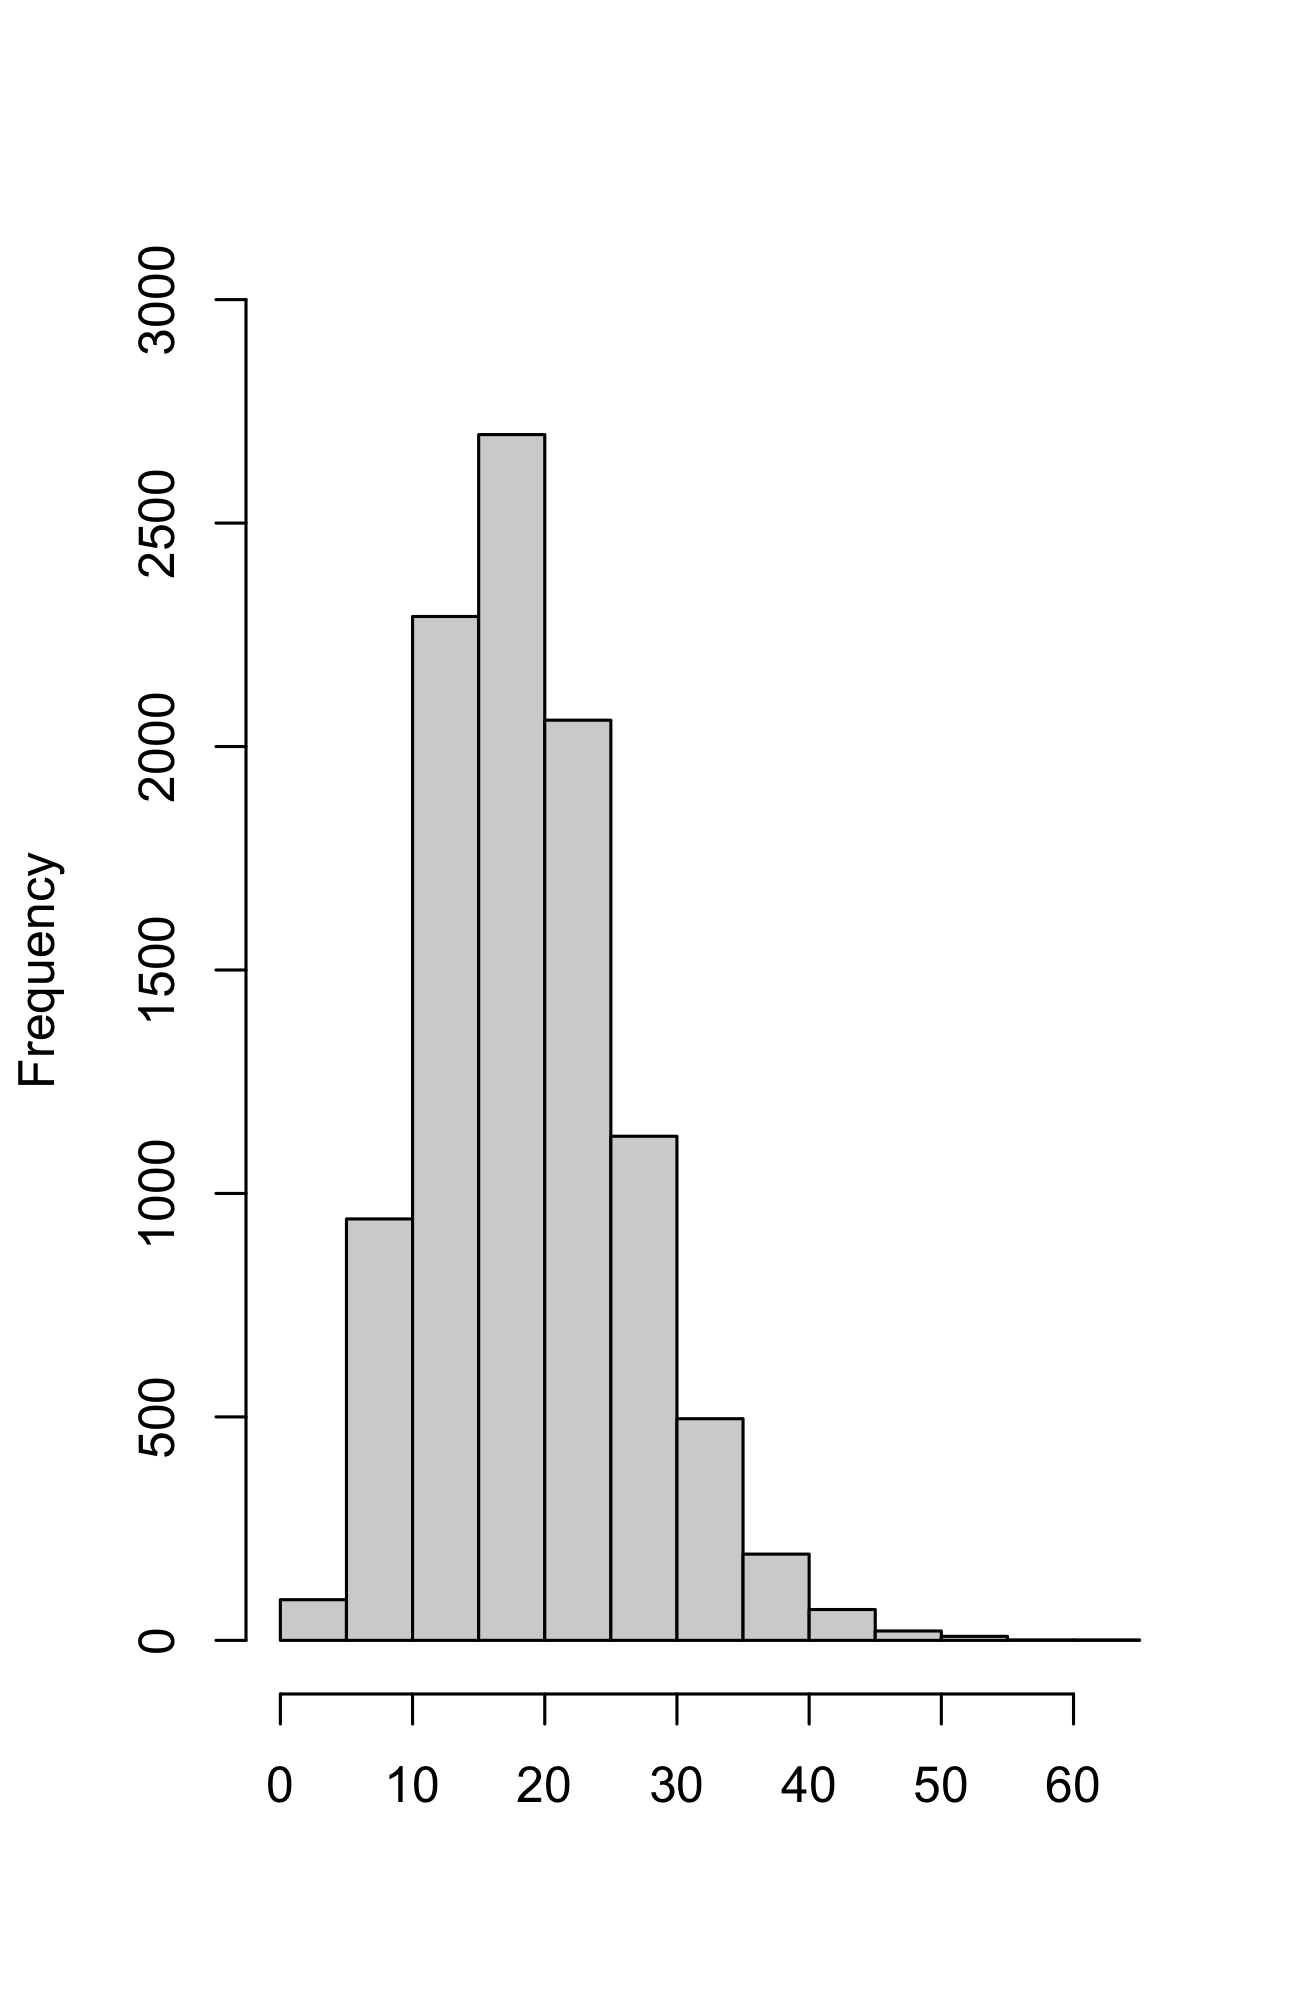
\includegraphics[width=.8\linewidth]{rbinom_bronte.png}  
  \caption{Using rbinom, Wuthering Heights.}
  \label{subfig6-3}
\end{subfigure}
\begin{subfigure}{.5\textwidth}
  \centering
  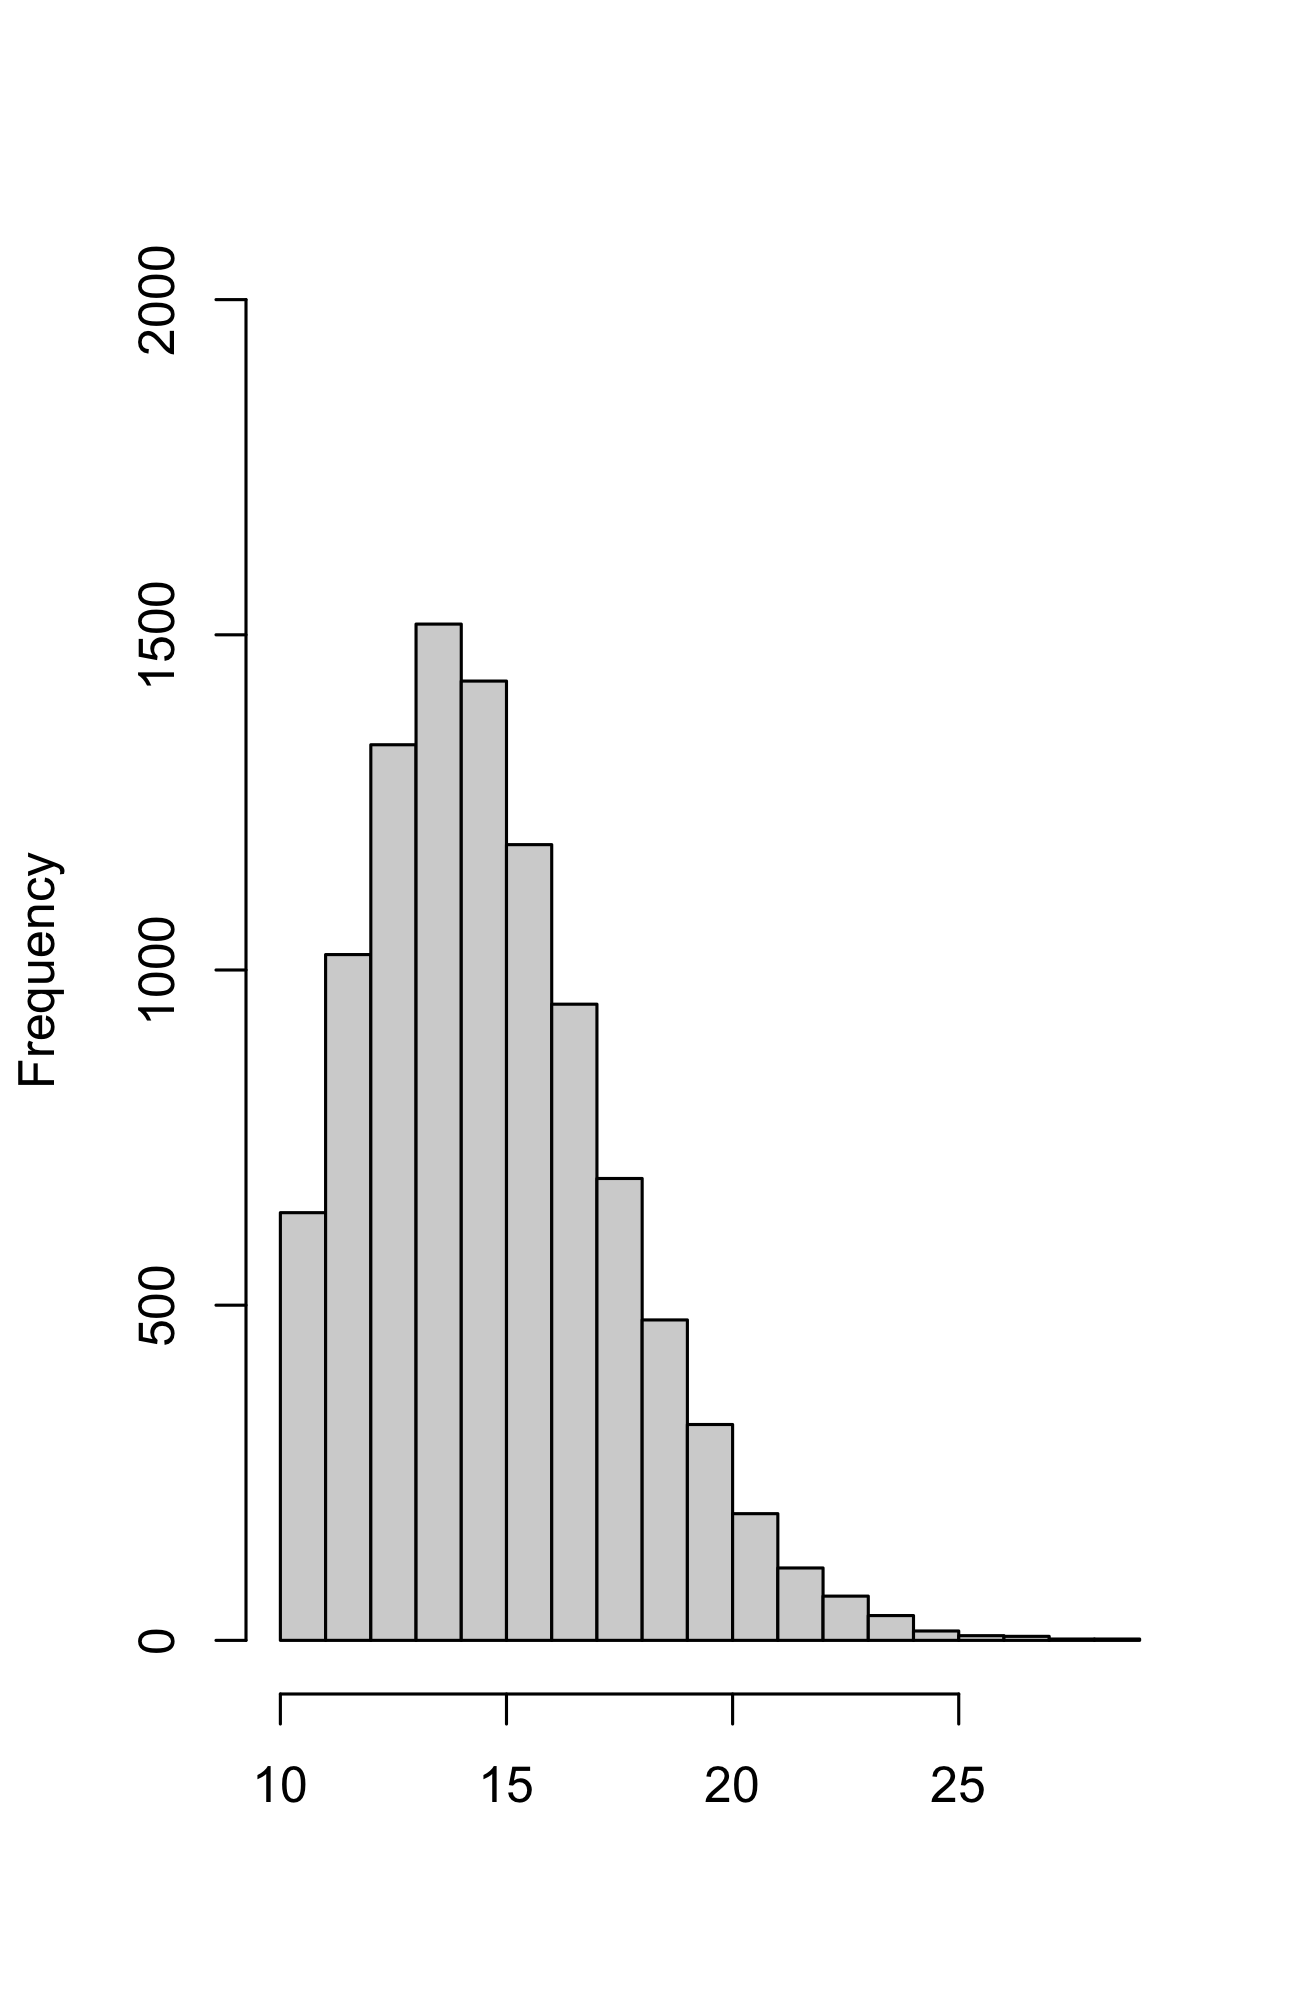
\includegraphics[width=.8\linewidth]{co_rbinom_bronte.png}  
  \caption{Using made code, Wuthering Heights.}
  \label{subfig6-4}
\end{subfigure}
\caption{Comparison between the use of the tool \texttt{rbinom}}
\label{fig6}
\end{figure}

In Figure \ref{fig6} we use now the \texttt{rbinom} \cite{rbinom} tool to further our experiments. This tool adds a variable inside the parameters. Same as with the \texttt{rgeom} tool, we have the number of experiments, then we have a number ($k$) which determines the amount of successful events before it can move to the next iteration. Then it needs the parameter of probability of success.\\

In Subfigures \ref{subfig6-1} and \ref{subfig6-3} we use the parameter of 10,000 iterations, with $k$ number equal to 10. The probability of success is 0.51 and 0.34 respectively. Then for the made code in both books we use the same parameters, but using our binary data of each book.\\

As we can appreciate in the comparison in Figure \ref{fig6} the behaviour of the plots is very similar.\\ 

For the last experimentation with distribution, we take the tool \texttt{rhyper} \cite{rhyper}. In this case, it requires the amount of iterations, the amount of \say{white balls}, the amount of \say{black balls} and the size of our sample. The white balls are represented as our positive words. The black balls as the negative ones. We set our iterations at 10,000 and our sample as 50.\\

Both tables have a gray and a white area. The gray area represents the number of bad words found in our sample of 50. The white area represents the number of times that many negative words repeated it self in our 10,000 iterations. In Table \ref{table2} we see the results of using the \texttt{rhyper} tool with the book Pride and Prejudice. Doing some calculations with our percentage of positive and negative words of this book, we have as a limit of negative words 24. So we add up all the frequencies after 24, and divide them for 10,000. The result of this is 0.4411. \\

Moving to Table \ref{table1} we have a different limit parameter. In this case is 33. So we add up all of the elements after the 33 and divide them by 10,000. The result is 0.4388.\\
.
\begin{table}\caption{Table of results from the \texttt{rhyper} tool with book Pride and Prejudice.}
\begin{center}\label{table2}
\begin{tabular}{ | c | c | c | c | c | c | c | c | c |}
\hline
\rowcolor{Gray}
11	&	12	&	13	&	14	&	15	&	16	&	17	&	18	&	19	\\
3	&	2	&	10	&	26	&	49	&	96	&	184	&	278	&	419	\\
\hline
\hline
\rowcolor{Gray}
20	&	21	&	22	&	23	&	24	&	25	&	26	&	27	&	28	\\
619	&	799	&	984	&	1036	&	1084	&	1101	&	892	&	818	&	596	\\
\hline
\hline
\rowcolor{Gray}
29	&	30	&	31	&	32	&	33	&	34	&	35	&	36	&	38	\\
429	&	276	&	143	&	84	&	43	&	24	&	2	&	2	&	1	\\
\hline
\end{tabular}
\end{center}
\end{table}


\begin{table}\caption{Table of results from the \texttt{rhyper} tool with book Wuthering Heights}
\begin{center}\label{table1}
\begin{tabular}{ | c | c | c | c | c | c | c | c | c |}
\hline
\rowcolor{Gray}
20	&	21	&	22	&	23	&	24	&	25	&	26	&	27	&	28	\\
2	&	2	&	8	&	27	&	41	&	86	&	145	&	258	&	417	\\
\hline
\hline
\rowcolor{Gray}
29	&	30	&	31	&	32	&	33	&	34	&	35	&	36	&	37	\\
566	&	786	&	977	&	1171	&	1126	&	1176	&	988	&	800	&	646	\\
\hline
\hline
\rowcolor{Gray}
38	&	39	&	40	&	41	&	42	&	43	&	44	&	45	&\cellcolor{white}		\\
375	&	213	&	109	&	50	&	17	&	8	&	5	&	1	&		\\
\hline
\end{tabular}
\end{center}
\end{table}

Now, for our self made code, we use the same parameters for each book, 10,000 iterations, $k$ of 10, and a sample of 50. The only variants are the positive and negative words for each book. Something else we added was the limit variable, which is the same as we used to make our calculation with the tables, 24 for Austen and 33 for Bront$\ddot{e}$. As a result we have, in the case of Austen a probability of 0.448 and 0.435 for Bront$\ddot{e}$. Comparing this to our results with the calculation of the tables we have 0.4411 and 0.4388, we have very similar results. \\



\section{Other experiments}

In the previous practice I struggled with word cloud plots. Here in Figure \ref{fig0} I make a comparison of positive and negative words in both books. I find it quite funny that the main words for each book are miss and master.\\~\\



\begin{figure}[]
\begin{subfigure}{.5\textwidth}
  \centering
  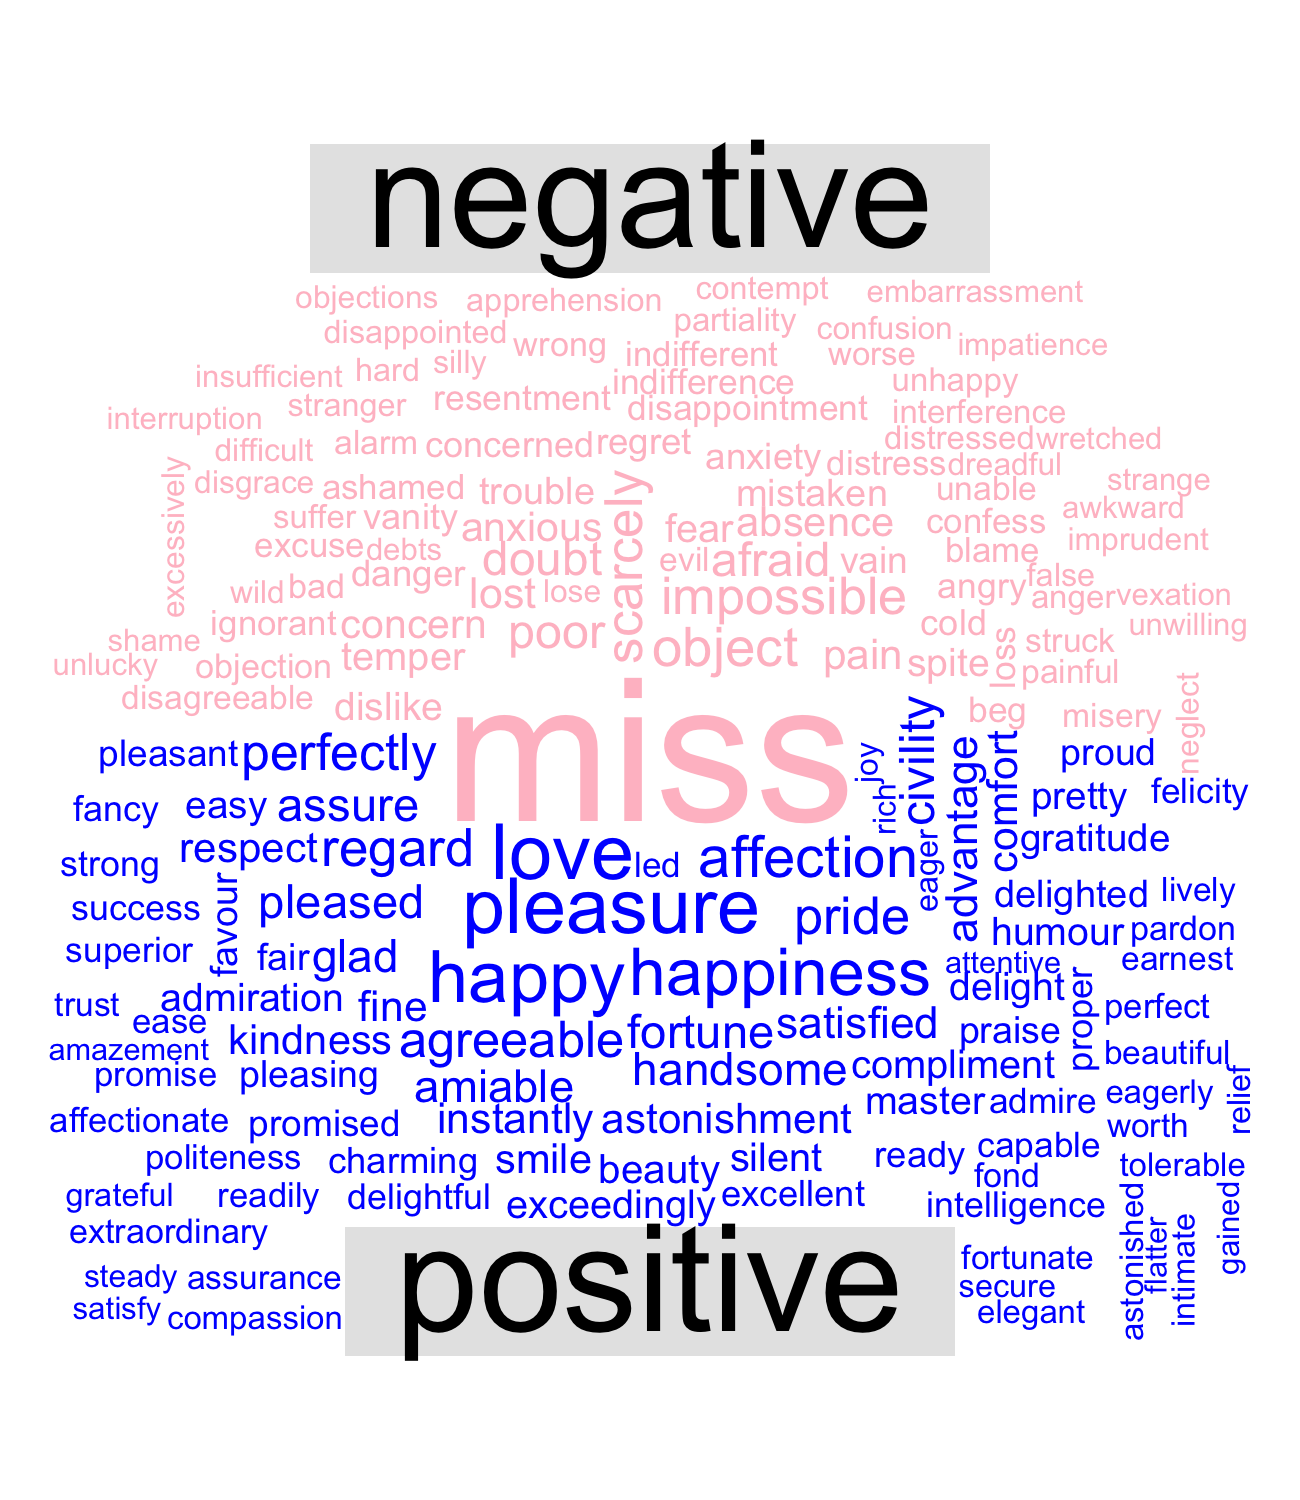
\includegraphics[width=1\linewidth]{word_austen.png}  
  \caption{Pride and Prejudice}
  \label{subfig0-1}
\end{subfigure}
\begin{subfigure}{.5\textwidth}
  \centering
  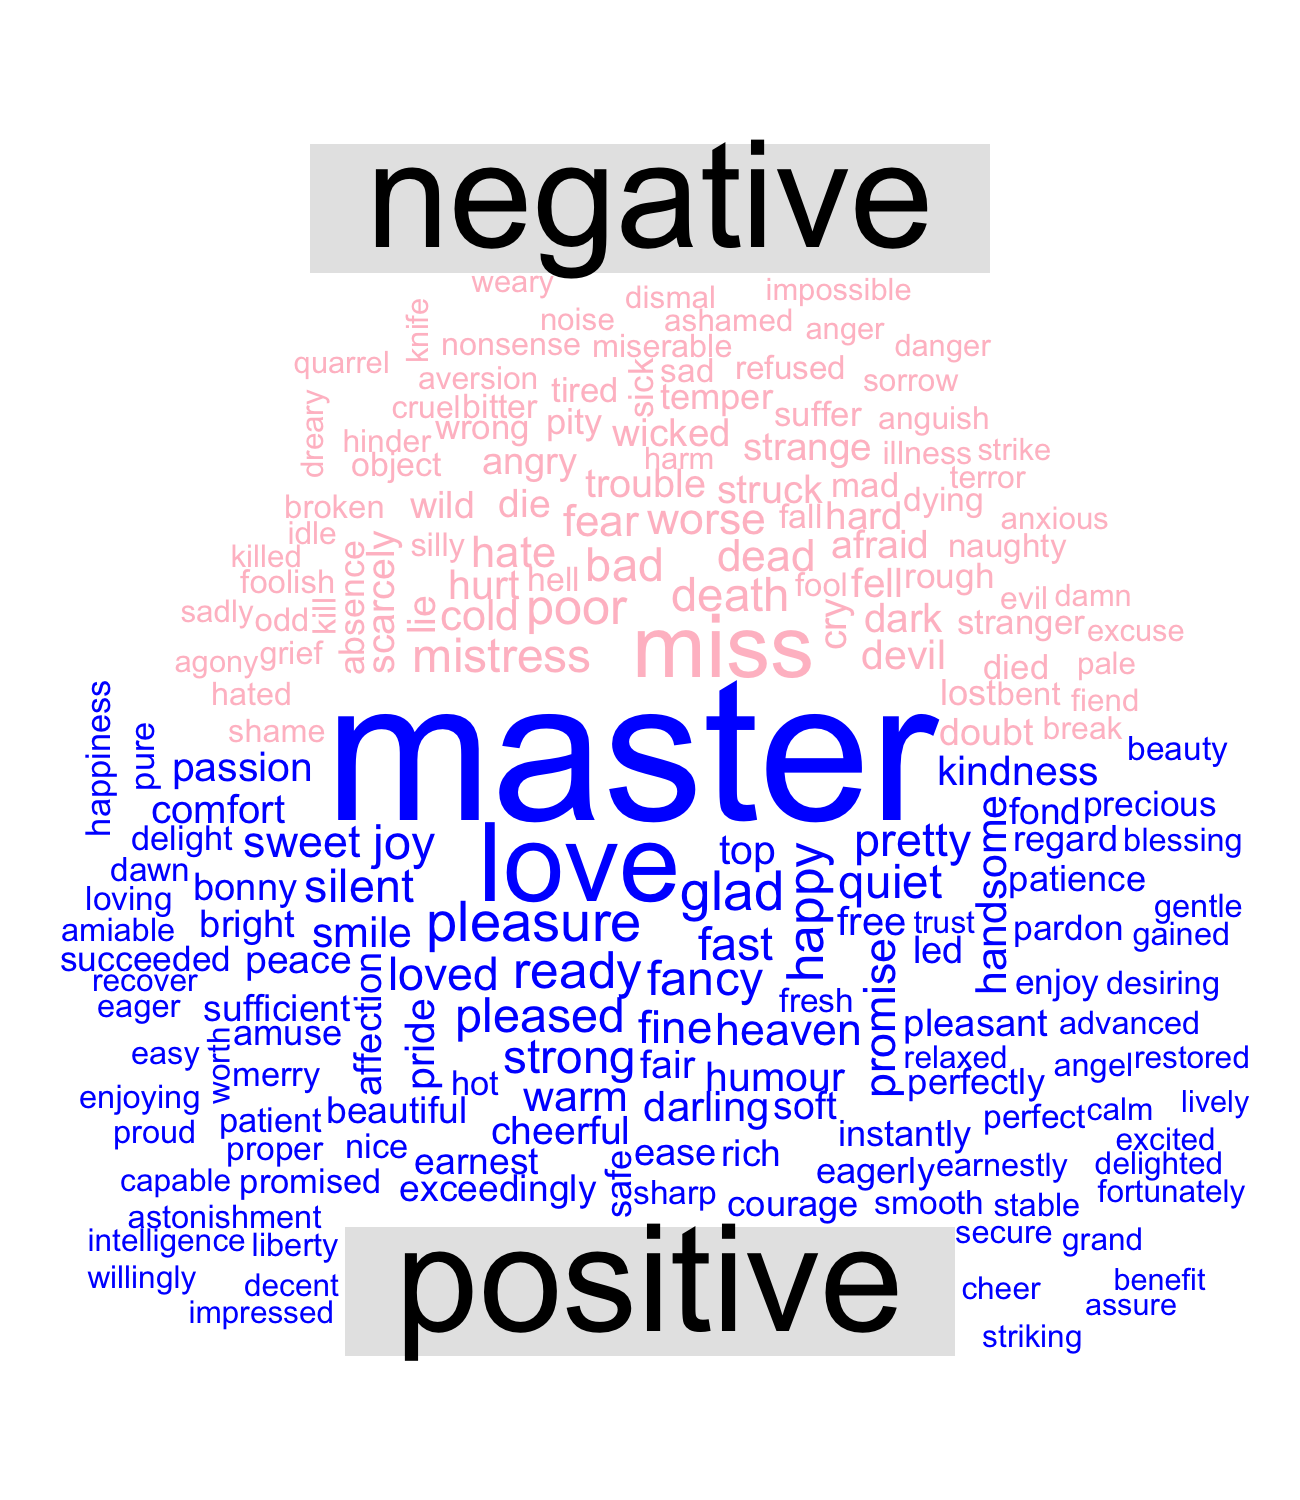
\includegraphics[width=1\linewidth]{word_bronte.png}  
  \caption{Wuthering Heights}
  \label{subfig0-2}
\end{subfigure}
\caption{Word cloud of positive and negative words in both books}
\label{fig0}
\end{figure}


\section{Conclusions}

With our first comparison of positive and negative distribution of words we were able to identify that Wuthering Heights has a more dark, more macabre tone of writing than Pride and Prejudice. The following plots with the R tools such as \texttt{rgeom, rbinom} and \texttt{rhyper} were interesting to develop in self made code. It was also curious to see the last experiment, and be able to prove again our impression on the difference of writing in both books. \\

In Tables \ref{table2} and \ref{table1} what sparked attention was the begining and end frequency of each. In Table \ref{table2} we begin with a small number and en with the number 38, with very low frequencies. This tells us that there is a small amount of negative words in this data. And in Table \ref{table1} we begin with frequency of 20 and end up in the number 45. This is also aligned with the percentage of the positive and negative words we know of the book.\\



\bibliographystyle{plainnat}
\bibliography{tarea3}


 
\end{document}